\documentclass[
    9pt,            % 8-20pt possible
    % twocolumn,      % switch, use twocolumn layout
    techreport,        % select between  ``techreport'', ``report'', ``article'', ``commun'', ``persp'' and ``review''
    % lineno,         % switch, adds line numbering
    % tocfig,         % switch, use a TOC figure at the top (place in ./figs)
    % SI,             % switch to Supplemental Information format, not compatible with twocolumn
    affiltop,       % switch, put affiliations under authors (instead of footnote)
    % nofootprint,    % do not add "Preprint" in footer
    % nofootdate,     % do not add date in footer
    % debug,          % switch, add debugging boxes
    % draft,          % for quick compilations (no figures, references etc)
]{art}


% Title
\newcommand{\pubtitle}{Geb Pipeline v5.0}

\newcommand{\pubauthA}{Artem Gureev}
\newcommand{\pubaffilA}{a}
% \newcommand{\orcidA}{0000-0001-5477-1503}
\newcommand{\authemailA}{artem@heliax.dev}
% \newcommand{\eqcontribA}{}

\newcommand{\pubauthB}{Jonathan Prieto-Cubides}
\newcommand{\pubaffilB}{a}
% \newcommand{\orcidB}{0000-0001-0000-0000}
\newcommand{\authemailB}{jonathan@heliax.dev}
% \newcommand{\eqcontribB}{}

% \newcommand{\pubauthC}{Last Author}
% \newcommand{\pubaffilC}{a}
% \newcommand{\orcidC}{0000-0001-5477-1503}
% \newcommand{\authemailC}{mail@someinstitute.com}

% Institutions/Affiliations
\newcommand{\pubaddrA}{%
Heliax AG }

% Corresponding author mail
\newcommand{\pubemail}{\authemailA}

\newcommand{\pubabstract}{
At Heliax, we are developing a compiler stack to facilitate the creation of
decentralized applications using high-level functional programming
languages. This stack comprises a series of compilers that begin with
Juvix and culminate in various targets. One such target is arithmetic circuits, represented via VampIR,
an intermediate language for such circuits. This report highlights the
Geb project, a component of this pipeline, and details the process of
compiling JuvixCore into VampIR through the Geb compiler. To aid
its adoption and implementation, we provide a categorical overview of the
mathematical foundations of the Geb project and insights into its
current Lisp-based implementation. The objective of this report is to guide
future implementations and improvements of the Geb project.
}

% Description of the SI file, placed as a footnote
% \newcommand{\pubSI}{Electronic Supplementary Information (ESI) available:
% one PDF file with all referenced supporting information.}

% Any keywords to be displayed under the abstract
\keywords{ 
Geb \sep%
Juvix \sep%
VampIR \sep%
compilers \sep%
category theory \sep%
semantics of PL \sep%
Lambda calculus \sep% 
Arithmetic circuits\sep}

% Supplementary space between title/abstract and text, if needed
% \newcommand{\pubVadj}{0pt}

% ! DO NOT REMOVE OR MODIFY !
%%%%%%%%%%%%%%%%%%%%%%%%%%%%%%%%%%%%%%%%%%%%%%%%%%%%%%%%%%%%%%%%%%%%%
%%%%%%%%%%%%%%%%%%%%%%%%%%%%%%%%%%%%%%%%%%%%%%%%%%%%%%%%%%%%%%%%%%%%%
%% In an PI manuscript the preamble contains
%%      - paper title
%%      - paper metadata (authors/affiliations...)
%%      - paper abstract
%%      - paper keywords
%%      - vertical space adjustment between text and abstract
%%%%%%%%%%%%%%%%%%%%%%%%%%%%%%%%%%%%%%%%%%%%%%%%%%%%%%%%%%%%%%%%%%%%%
%%%%%%%%%%%%%%%%%%%%%%%%%%%%%%%%%%%%%%%%%%%%%%%%%%%%%%%%%%%%%%%%%%%%%


%%%%%%%%%%%%%%%%%%%%%%%%%%%%%%%%%%%%%%%%%%%%%%%%%%%%%%%%%%%%%%%%%%%%%
%% Title
%% -----
%%%%%%%%%%%%%%%%%%%%%%%%%%%%%%%%%%%%%%%%%%%%%%%%%%%%%%%%%%%%%%%%%%%%%
\title{\pubtitle}

%%%%%%%%%%%%%%%%%%%%%%%%%%%%%%%%%%%%%%%%%%%%%%%%%%%%%%%%%%%%%%%%%%%%%
%% Meta-data block
%% ---------------
%%%%%%%%%%%%%%%%%%%%%%%%%%%%%%%%%%%%%%%%%%%%%%%%%%%%%%%%%%%%%%%%%%%%%

\newcommand{\dg}{\textsuperscript{\textbf{\dag\textnormal{,}}}}

\ifdef{\pubauthA}{\author[\pubaffilA]{\pubauthA\ifdef{\orcidA}{~\protect\orcid{\orcidA}}{}\ifdef{\eqcontribA}{\dg}{}}}{}
\ifdef{\pubauthB}{\author[\pubaffilB]{\pubauthB\ifdef{\orcidB}{~\protect\orcid{\orcidB}}{}\ifdef{\eqcontribB}{\dg}{}}}{}
\ifdef{\pubauthC}{\author[\pubaffilC]{\pubauthC\ifdef{\orcidC}{~\protect\orcid{\orcidC}}{}\ifdef{\eqcontribC}{\dg}{}}}{}
\ifdef{\pubauthD}{\author[\pubaffilD]{\pubauthD\ifdef{\orcidD}{~\protect\orcid{\orcidD}}{}\ifdef{\eqcontribD}{\dg}{}}}{}
\ifdef{\pubauthE}{\author[\pubaffilE]{\pubauthE\ifdef{\orcidE}{~\protect\orcid{\orcidE}}{}\ifdef{\eqcontribE}{\dg}{}}}{}
\ifdef{\pubauthF}{\author[\pubaffilF]{\pubauthF\ifdef{\orcidF}{~\protect\orcid{\orcidF}}{}\ifdef{\eqcontribF}{\dg}{}}}{}
\ifdef{\pubauthG}{\author[\pubaffilG]{\pubauthG\ifdef{\orcidG}{~\protect\orcid{\orcidG}}{}\ifdef{\eqcontribG}{\dg}{}}}{}
\ifdef{\pubauthH}{\author[\pubaffilH]{\pubauthH\ifdef{\orcidH}{~\protect\orcid{\orcidH}}{}\ifdef{\eqcontribH}{\dg}{}}}{}
\ifdef{\pubauthI}{\author[\pubaffilI]{\pubauthI\ifdef{\orcidI}{~\protect\orcid{\orcidI}}{}\ifdef{\eqcontribI}{\dg}{}}}{}
\ifdef{\pubauthJ}{\author[\pubaffilJ]{\pubauthJ\ifdef{\orcidJ}{~\protect\orcid{\orcidJ}}{}\ifdef{\eqcontribJ}{\dg}{}}}{}
\ifdef{\pubauthK}{\author[\pubaffilK]{\pubauthK\ifdef{\orcidK}{~\protect\orcid{\orcidK}}{}\ifdef{\eqcontribK}{\dg}{}}}{}

\ifdef{\eqcontribA}{\equalcontrib{}}{}
\ifdef{\eqcontribB}{\equalcontrib{}}{}
\ifdef{\eqcontribC}{\equalcontrib{}}{}
\ifdef{\eqcontribD}{\equalcontrib{}}{}
\ifdef{\eqcontribE}{\equalcontrib{}}{}
\ifdef{\eqcontribF}{\equalcontrib{}}{}
\ifdef{\eqcontribG}{\equalcontrib{}}{}
\ifdef{\eqcontribH}{\equalcontrib{}}{}
\ifdef{\eqcontribI}{\equalcontrib{}}{}
\ifdef{\eqcontribJ}{\equalcontrib{}}{}
\ifdef{\eqcontribK}{\equalcontrib{}}{}

\ifdef{\pubaddrA}{\affil[a]{\pubaddrA}}{}
\ifdef{\pubaddrB}{\affil[b]{\pubaddrB}}{}
\ifdef{\pubaddrC}{\affil[c]{\pubaddrC}}{}
\ifdef{\pubaddrD}{\affil[d]{\pubaddrD}}{}
\ifdef{\pubaddrE}{\affil[e]{\pubaddrE}}{}
\ifdef{\pubaddrF}{\affil[f]{\pubaddrF}}{}
\ifdef{\pubaddrG}{\affil[g]{\pubaddrG}}{}
\ifdef{\pubaddrH}{\affil[h]{\pubaddrH}}{}

\contact{\pubemail}

%%%%%%%%%%%%%%%%%%%%%%%%%%%%%%%%%%%%%%%%%%%%%%%%%%%%%%%%%%%%%%%%%%%%%
%% Abstract
%% --------
%%%%%%%%%%%%%%%%%%%%%%%%%%%%%%%%%%%%%%%%%%%%%%%%%%%%%%%%%%%%%%%%%%%%%

\begin{abstract}
    \pubabstract{}
\end{abstract}

%%%%%%%%%%%%%%%%%%%%%%%%%%%%%%%%%%%%%%%%%%%%%%%%%%%%%%%%%%%%%%%%%%%%%
%% Keywords
%% --------
%%%%%%%%%%%%%%%%%%%%%%%%%%%%%%%%%%%%%%%%%%%%%%%%%%%%%%%%%%%%%%%%%%%%%

\ifdef{\pubkeywords}{\keywords{\pubkeywords}}{}

%%%%%%%%%%%%%%%%%%%%%%%%%%%%%%%%%%%%%%%%%%%%%%%%%%%%%%%%%%%%%%%%%%%%%
%% Adjusting vertical space
%% ------------------------
%%%%%%%%%%%%%%%%%%%%%%%%%%%%%%%%%%%%%%%%%%%%%%%%%%%%%%%%%%%%%%%%%%%%%

\ifdef{\pubVadj}{\verticaladjustment{\pubVadj}}{}

% The preprint DOI to be used as an link in the paper
\pubdoi{10.5281/zenodo.8262747}
\history{(Received August 8, 2023; Published: August 22, 2023)}
% MACROS
\newcommand{\N}{\mathbb{N}}
\usepackage{parskip}
\usepackage{minted}
\usepackage[most]{tcolorbox}
\colorlet{LightLavender}{gray!40!}
\tcbset{on line, 
        boxsep=0pt, left=1pt,right=1pt,top=1pt,bottom=1pt,
        colframe=white,colback=LightLavender,  
        highlight math style={enhanced}
        }

\newcommand{\gebinit}{\tcbox{\normalfont{so0}}}
\newcommand{\gebterm}{\tcbox{\normalfont{so1}}}
\newcommand{\gebcoprod}{\tcbox{\normalfont{coprod}}}
\newcommand{\gebprod}{\tcbox{\normalfont{prod}}}
\newcommand{\gebobj}{\tcbox{\normalfont{substobj}}}
\newcommand{\gebmorph}{\tcbox{\normalfont{substmorph}}}
\newcommand{\lamerr}{\tcbox{\normalfont{err}}}

\newcommand{\SeqN}{\ensuremath{\mathsf{Seq}\N}}
\newcommand{\FinSet}{\ensuremath{\mathsf{FinSet}}}
\newcommand{\FinOrd}{\ensuremath{\mathsf{FinOrd}}}
\newcommand{\JuvixCore}{\ensuremath{\mathsf{JuvixCore}}}
\newcommand{\Geb}{\ensuremath{\mathsf{Geb}\,}}
\newcommand{\Juvix}{\ensuremath{\mathsf{Juvix}}}
\newcommand{\VampIR}{\ensuremath{\mathsf{VampIR}}}
\newcommand{\LambdaIR}{\ensuremath{\mathsf{Lambda}}}


\begin{document}

\maketitle
\iftoggle{SI}{}{\ifdef{\pubSI}{\footnotetext{\pubSI}}{}}

\tableofcontents

\section{Introduction}

The \Geb{} project was initiated to compile functional programs into
high-level representations of arithmetic circuits using categorical
methods. This categorical approach specifies compilation procedures via
internal language theorems, thus shifting focus from syntax to suitable
categorical structures.

The core of the approach taken here rests on the observation that
compilation procedures\footnote{Those that preserve specified type structures.} can be linked to
functors that maintain the corresponding structures between categories
representing appropriate programming languages.  One canonical example is
specified in~\cite{LS-catlog}, dealing with the fact that 
languages possessing the simply typed Lambda calculus (STLC) structure form a
category which is equivalent to the category of Cartesian Closed Categories
(CCC).

Therefore, instead of operating with syntax, we can represent our languages
as categories and construct functors between them as also described in~\cite{elliot-categories}. This approach simplifies compiler
formalization due to the direct mathematical meaning of the constructions.
Furthermore, functor properties inherently provide several beneficial
features, including automatic type-checking for morphism composition.

The approach outlined in this document is supported by a reference
implementation in Lisp. This Lisp-based \Geb{} implementation signifies the
project's initial completed stage: the compilation of functional programs
written in the \JuvixCore{} language (regarded as an appropriate untyped
Lambda calculus with optional typing) to \VampIR{}, an in-house language
for arithmetic circuits. As part of the implementation, we also provide an
interactive user environment equipped with extra features such as
interpreters, program type-checkers, and a \Geb{} visualizer available at
the following address, release v0.5.
\begin{center}
    \url{https://github.com/anoma/geb}.
\end{center}

The general aim of the paper is to provide an overview of pipeline design
that is accessible to people without delving deep in the Lisp implementation.
Primarily, we aim to:

\begin{enumerate}
\item Make all components of the pipeline precise by describing their
intended semantics and paraphrasing the constructions in ML-like code with
explicit typing.
\item Describe all the compilation steps using diagrams for readability and
intelligibility.
\item  Highlight important interactive features of the current
implementation (see \Cref{appendix:interactive-lisp}).
\end{enumerate}

\section{Language/Category Specs}

The central challenge is to effectively specify the compilation of
programs, written in a high-level functional programming language, into an
intermediate arithmetic circuit language. Here, this corresponds to the
translation from \Juvix{} to the \VampIR{} language, with a specific focus
on the compilation of \JuvixCore{} to \VampIR{}.
% https://q.uiver.app/#q=WzAsMyxbMCwwLCJcXEp1dml4e30iXSxbMywxLCJcXFZhbXBJUnt9Il0sWzMsMCwiXFxKdXZpeENvcmV7fSJdLFswLDEsIiIsMCx7InN0eWxlIjp7ImJvZHkiOnsibmFtZSI6ImRhc2hlZCJ9fX1dLFswLDJdLFsyLDFdXQ==

\[\begin{tikzcd}
    {\Juvix{}} &&& {\JuvixCore{}} \\
    &&& {\VampIR{}}
    \arrow[dashed, from=1-1, to=2-4]
    \arrow[from=1-1, to=1-4]
    \arrow[from=1-4, to=2-4]
\end{tikzcd}\]

\begin{itemize}
  \item \JuvixCore{}: A Lambda calculus (with possible typing)
  incorporating inductive types and primitive integers, which defines the
  strict execution semantics of \Juvix{}.
  \item \VampIR{}: An intermediate language for arithmetic circuit
  specification, akin to LLVM IR. It features useful constructors such as
  tuples, arrays, mapping and folds, currying, and circuit synthesis to
  Plonkup and Halo2.
\end{itemize}

The first step in this is to provide a compilation from a sub language of
\Juvix{}, namely \JuvixCore{}. The way we do this is by breaking up the
procedure into compilations through languages we name \LambdaIR{}, \Geb{},
and \SeqN{}.

% https://q.uiver.app/#q=WzAsNSxbMCwwLCJcXG5vcm1hbHtKdXZpeCBDb3JlfSJdLFsyLDAsIlxcdGV4dHtMYW1iZGF9Il0sWzQsMCwiXFx0ZXh0e0dlYn0iXSxbNiwwLCJcXHRleHR7U2VxJFxcTiR9ICJdLFs4LDAsIlxcdGV4dHtWYW1wLUlSfSJdLFsxLDJdLFsyLDNdLFszLDRdLFswLDFdXQ==
\[\begin{tikzcd}
    {\JuvixCore{}} && {\LambdaIR{}} && {\Geb{}} && {\text{\SeqN{}} } && {\VampIR{}}
    \arrow[from=1-3, to=1-5]
    \arrow[from=1-5, to=1-7]
    \arrow[from=1-7, to=1-9]
    \arrow[from=1-1, to=1-3]
\end{tikzcd}\]

Here we are concerned only with the steps starting from \LambdaIR{}. The
\Juvix{} compiler already supports compiling \JuvixCore{} to a suitable
representation in \LambdaIR{}. Hence, the pipeline we will be interested in
and the one written in Lisp is presented in the diagram below.

% https://q.uiver.app/#q=WzAsNCxbMCwwLCJcXHRleHR7TGFtYmRhfSJdLFsyLDAsIlxcdGV4dHtHZWJ9Il0sWzQsMCwiXFx0ZXh0e1NlcSRcXE4kfSAiXSxbNiwwLCJcXHRleHR7VmFtcC1JUn0iXSxbMCwxXSxbMSwyXSxbMiwzXV0=
\[\begin{tikzcd}
    {\LambdaIR{}} && {\Geb{}} && {\SeqN{}} && {\VampIR{}}
    \arrow[from=1-1, to=1-3]
    \arrow[from=1-3, to=1-5]
    \arrow[from=1-5, to=1-7]
\end{tikzcd}\]

The current section is devoted to the specifications of the languages used
in the compilation with the \VampIR{} section concerned not with the
description of \VampIR{} itself, but of the library of functions needed for
any compiled code to compile on valid inputs.

Let us provide a summary of the language features of each language in the
compiler stack, as originally presented in \cite{lukascz-vampir}.

\vspace*{2mm}
\begin{minipage}[b]{\hsize}\centering
\begin{tabular}{lllll}
\hline
\textbf{Feature} & \textbf{\Juvix{}} & \textbf{\JuvixCore{}} & \textbf{\Geb{}} & \textbf{\VampIR{}} \\ \hline
General recursion (functions)   &  Yes   &  Yes   &  No  &   No  \\
First-class functions   &  Yes   &  Yes   &  Yes  &   No\footnote{\VampIR{} higher-order and anonymous functions are not fully ``first-class'' because they cannot nontrivially interact with the field elements - they are essentially compilation-time-only.}  \\
Inductive data types  &  Yes   &  Yes   &  No  &   No  \\
Finite data structures  &  Yes   &  Yes   &  Yes & No\footnote{Pairs and lists in \VampIR{} cannot nontrivially interact with the field elements. In general, finite \JuvixCore{} data structures cannot be translated into them.}  \\
Prenex polymorphism  &  Yes   &  Yes   &  No  &  No\footnote{Polymorphic functions are supported, but not polymorphic data types which can interact non-trivially with field elements. Hence, monomorphisation is still necessary to translate from \JuvixCore{}.} \\
Higher-rank polymorphism  &  Some   &  Yes   &  No  &   No  \\
Primitive integer type  &  Yes   &  Yes   &  Yes  &   Yes\footnote{\VampIR{} ``integers'' are the field elements, not integers strictly speaking.} \\
Errors &  Yes   &  Yes   &  Yes  &   No \\
\hline
\end{tabular}
% \caption{Language features}
\end{minipage}


\subsection{Geb}

The finite version of \Geb{} implemented here answers two questions:
\begin{itemize}
    \item What are the minimal/optimal operations needed to present
    polynomials which \VampIR{} operates with?
    \item What are the minimal/optimal bounding operations between
    functional programming languages?
\end{itemize}
The answer seems to be that we need some sort of addition, multiplication,
$0$, and $1$ as structures to be used. For the usual arithmetic to hold, we
also need some sort of distributivity law. Exponentiation should follow in
a similar fashion to how we define arithmetic exponentiation from
multiplication in $\N$\footnote{Of course multiplication can be defined
similarly by addition, but it is not optimal to do so due to exponentiation
of terms. Moreover, it seems that having primitive exponentiation in a
language through which we compile is inefficient, as it would need to
compile to some separate \VampIR{} function.}. Finally, we need some notion
of a "context" or a "domain" - as is usual in the syntax/semantics duality
- in order to be able to produce variables.

Hence, this brings us to the first definition of \Geb{}.

\begin{definition}\label{def:geb1} \Geb{} is the language spanned by the
empty type \tcbox{\normalfont{so0}}, unit type \gebterm \, and
sum/product types appropriately named \gebcoprod \,  and \gebprod.
\end{definition}

%NOTE: For readibility makes sence to rename substmorph to some infix notation expressing arrows, otherwise it may be confusing to a lot of people

Here is a definition as one would write using Agda-like syntax:

\begin{minted}{agda}
data substobj : Set where
  so1 : substobj
  so0 : substobj
  coprod : substobj → substobj → substobj
  prod : substobj → substobj → substobj

variable
    x y z : substobj

data _G→_ : substobj → substobj → Set where
   comp : (y G→ z) → (x G→ y) → (x G→ z)
   -- composition
   id : (x : substobj) → (x G→ x)
   -- identity function
   initial : (x : substobj) → (so0 G→ x)
   -- absurd
   terminal : (x : substobj) → (x G→ so1)
   -- constant function
   mcase : (x G→ z) → (y G→ z) → ((coprod x y) G→ z)
   -- casing
   prod  : (z G→ x) → (z G→ y) → (z G→ (prod x y))
    -- product analysis
   distribute : (prod x (coprod y z)) G→ (coprod (prod x y) (prod x z))
    -- distributivity
   →left : x G→ (coprod x y)
    -- left injection
   →right : y G→ (coprod x y)
    -- right injection
   ←left : (prod x y) G→ x
    -- left projection
   ←right : (prod x y) G→ y
    -- right projection

subtmorph : substobj → substobj → Set
substmorph a b = a G→ b
\end{minted}

\begin{remark}
In the implementation, we use the name \tcbox{substmorph} for the type
above but for readability we use \tcbox{G→} here.
\end{remark}

Here \gebobj is the collection of the types of our language and \tcbox{f :
substmorph a b} stands for a term of \tcbox{b} in the context of \tcbox{a}\footnote{There are extra equalities to subject the terms to,
e.g. making terminal terms unique or composition associative on the nose,
yet for the sake of the current project, we do not implement these, and if
needed, reductions are done by hand. There is also an explicit reducer in
development.}.

Another way of thinking about \Geb{} is to specify the categorical
structure instead of the syntactical one.

\begin{definition}\label{def:geb2} \Geb{} is the category freely spanned by
an initial object, terminal object, and finite (co)products alongside the
distributivity law.
\end{definition}

\begin{remark}
    The discussion below uses a more advanced categorical vocabulary.
    Anyone satisfied by the previous two definitions can instead go
    directly to \Cref{cor:CCC}.
\end{remark}

Recall that a category of models of a language is a category in which
objects are models of said language and morphisms are mappings that
maintain the language structure\footnote{For example, the category of
models of groups is the category of groups and group morphisms.}.
\cref{def:geb2} is equivalent to considering the term model of a language, which
is the initial category of its corresponding category of
models\footnote{For more abstract nonsense on the topic one can consult
\cite{K-L-hottt} and \cite{adamek_rosicky_1994}.}.

However, the semantics of \Cref{def:geb2} are unclear. Note that taking
coproducts with $\gebinit$ is equivalent to the identity
functor\footnote{Similar to how adding $0$ is the same as the identity
function.} while taking products with $\gebinit$ to a constant functor at
$\gebinit$\footnote{Distributive categories have strict initial objects,
similar to how multiplying by $0$ gives $0$.}. Similarly, taking products
with $\gebterm$ is equivalent to the identity functor\footnote{Similar to
how multiplying by $1$ gives back the original term.}. Therefore,
intuitively, the only way to make "new" types in \Geb{} is by taking
coproducts of $\gebterm$ with itself over and over. There is actually a
category which is specified by being generated by filtered colimits over
finite inclusions between such coproducts of the terminal object:
\FinSet{}. It is indeed generated by simply adding extra $1$-element sets
to the empty set. Thus, there is the third definition of \Geb{}.

\begin{definition}\label{def:geb3} \Geb{} is \FinSet{}.
\end{definition}

Let us make this correspondence exact:

\begin{theorem}
\FinSet{} is an initial weak model of the \Geb{} language. That is, it is
equivalent to the initial model of the essentially algebraic theory of
category theory with initial, terminal objects, finite (co)products
structure, and distributivity. Moreover, the equivalence preserves all
relevant categorical structure.
\end{theorem}

\begin{proof}
We can instead deal with the skeleton $Sk(\FinSet{}) = \FinOrd{}$, the
category of finite ordinals, since clearly the equivalence preserves all
relevant structure. Now suppose that $(C, 1_C, 0_C, +_C, \times_C)$ is a
distributive category with initial/terminal object.

Note that $(\bigoplus_{n} 1_C) \times_C (\bigoplus_m 1_C) = \bigoplus_{n
\times m} 1_C$ by induction on $n$.
\begin{itemize}
    \item When $n=0$ since the initial object is strict, then the product
    is just $0_C$ which is also the null coproduct.
    \item For the inductive step, consider the chain of isomorphisms below.
    \begin{align*}
\bigoplus_{1+n} 1_C \times_C \bigoplus_{m} 1_C &\cong \left(\bigoplus_n 1_C +_C 1_C\right) \times_C \bigoplus_m 1_C   \\
&\cong \left(\bigoplus_n 1_C \times_C \bigoplus_m 1_C\right)  +_C  \bigoplus_m 1_C  &\text{(By distributivity prop.)} \\
&\cong \bigoplus_{n \times m} 1_C + \bigoplus_m 1_C &\text{(By induction hypothesis on $n$)}\\
&\cong \bigoplus_{(1+n) \times m} 1_C .
\end{align*}
\end{itemize}

Now we prove that \FinOrd{} is our weakly initial model. To do so, we need
to construct a functor of type $\FinOrd{} \to C$ that preserves our
structure, and we also need to prove that it is unique up to a natural
isomorphism.

First, we construct the functor.

Recall that both \FinSet{} and \FinOrd{} constitute the weakly initial
category of the theory of categories with finite coproduct on one
object\footnote{\url{https://ncatlab.org/nlab/show/FinSet\#universal_properties}}.
Given that $C$ has coproducts and $1_C$, we can hence construct the functor
$F \colon \FinOrd{} \to C$, which preserves this structure along with the
terminal object. We claim that $F$ is our needed functor. We claim that the
product structure is also preserved. Given $n \times m$ proceed by
induction on $n$:

\begin{itemize}
    \item If $n= 0$, then we have
         $$F(0 \times m) = F(0) \cong 0_C \cong 0_C \times_C F(m) \cong
         F(0) \times_C F(m).$$
    \item For the inductive step, we use the previous observation:

\begin{align*}
    F((1+n) \times m) &= F((n \times m) + m) \\
    &\cong (F(n) \times_C F(m)) +_C F(m) &\text{(By induction and $F$ preserves coproducts)} \\
    &\cong \left(\bigoplus_n 1_C \times_C \bigoplus_m 1_C\right) +_C \bigoplus_m 1_C &\text{(By definition of $F$)}\\
    &\cong \bigoplus_{n \times m} 1_C + \bigoplus_m 1_C \\
    &\cong \bigoplus_{(1+n) \times m} 1_C \\
    &\cong \bigoplus_{1+n} 1_C \times_C \bigoplus_m 1_C \\
    &\cong F(1+n) \times F(m).
\end{align*}
\end{itemize}

Since everything the functor hits is a coproduct of the terminal object up
to an isomorphism and $F$ preserves all coproduct structure, it preserves
all other morphism structure, including product universal morphisms and
distributivity, that is, it is an actual functor of models.

The only thing left to prove is the uniqueness property of $F$.

However, by the same argument, since everything the functor hits is a
coproduct of $1_C$ and $F$ preserves coproduct structure and is a unique
functor doing so up to natural iso, this also proves uniqueness up to
iso.\qedhere
\end{proof}

Hence, \Cref{def:geb3} is fully valid and when one talks of \Geb{}, one can
instead think about a nice presentation of \FinSet{}. Hence a term of
$\gebobj$ is just a finite set and a term of \tcbox{\texttt{a G→ b}} is
just a function between corresponding finite sets. As expected, this
equivalence actually provides us with the existence of a lot of extra
structure.

\begin{corollary}\label{cor:CCC} Geb is cartesian closed.
\end{corollary}

That is, for any two objects \tcbox{a, b : substobj} we get an object
\tcbox{(sohomobj a b) : substobj} which is an object of \Geb{} representing
all terms of \tcbox{b} in context \tcbox{a}, or, in other words, it is the
function type from type \tcbox{a} to type \tcbox{b}. It also comes equipped
with the usual curry isomorphism and evaluation maps:

\begin{minted}{agda}
  curry : ((prod x y) G→ z) → (x G→ (sohomobj y z))
  eval : (prod (sohomobj x y) x) → y
  uncurry : (x G→ (sohomobj y z)) → ((prod x y) G→ z)
\end{minted}

\begin{remark}
The actual implementation of the said types and terms is not important for the report,
but we need these functions in order to compile \JuvixCore{}
code to \Geb{}, which is why these are mentioned. For explicit
constructions, one can consult the Agda
folder\footnote{\url{https://github.com/anoma/geb/blob/main/geb-agda/Geb_Hom.pdf}}.
\end{remark}

Now we "extend" \Geb{} by adding natural numbers with the following trick:
consider all $n$-bit-wide numbers. Evidently, there are $2^n$ of these,
which means that their set is in bijection with the finite ordinal of
cardinality $2^n$. In other words, we introduce objects \tcbox{nat-width n} for
every $n > 0$ which are really just isomorphic copies of $2^n$ coproducts
of $\gebterm$. So \Geb{} already had the natural number functionality, it
was just highly inefficient before introducing primitive constructors.

\begin{minted}{agda}
data substobj : Set where
...
  nat-width : Nat → substobj
  -- nat-width n is the set of n-bit natural numbers

data substmorph : substobj → substobj → Set where
  ...
  nat-add : (n : Nat) → ((nat-width n) G→ (nat-width n))
  -- addition
  nat-mult : (n : Nat) → ((nat-width n) G→ (nat-width n))
  -- multiplication
  nat-sub : (n : Nat) → (nat-width n)  G→  (nat-width n)
  -- subtraction
  nat-div : (n : Nat) → (nat-width n)  G→ (nat-width n)
  -- division
  nat-concat : (n m : Nat) → ((prod (nat-width n) (nat-width m))
                              G→ (nat-width (n+m)))
  -- concatenation of bits
  nat-inj : (n : Nat) → ((nat-width n) G→ (nat-width (n + 1)))
  -- injects an n-bit numbers as an n+1 bit number
  nat-decompose : (n : Nat) → ((nat-width (n + 1))
                               G→ (prod (nat-width 1) (nat-width n)))
  -- decomposes an n+1 bit number into the top bit and the rest of the bits
  one-bit-to-bool : (nat-width 1) G→ (coprod so1 so1)
  -- isomorphism between a set containing 0,1 bits and bool
  nat-eq : (n : Nat) → ((prod (nat-width n) (nat-width n))
                        G→ (coprod so1 so1))
  --equality predicate
  nat-lt : (n : Nat) → ((prod (nat-width n) (nat-width n))
                        G→ (coprod so1 so1))
  --"less-than" predicate
\end{minted}


\begin{remark}
Be careful when using the term "Geb" as it can point to many things. The
\Geb{} language, as it is currently implemented in the pipeline, is just a
subcomponent of what the final version of \Geb{} will look like. The
intention is that \Geb{} will become a language that will be able to
articulate the entirety of the pipeline currently presented in CL. The
reason we call this category \Geb{} here is that this category will be a
core component specifying the higher-order \Geb{} category, which itself
will correspond to a larger programming language. However, in this report
we always use "Geb" to describe \Geb{} as given
in~\Cref{def:geb1,def:geb2,def:geb3}.
\end{remark}

\begin{comment}
\begin{remark}
Note that while the code written for Geb has the same intended semantics as
its Lisp implementation, it is indeed different. The Lisp code is untyped.
Also note that $\tcbox{id}$ is not an actual function in the Lisp
implementation, instead we use just the names of the objects.
\end{remark}
\end{comment}

\subsection{\large\LambdaIR{}}

The \LambdaIR{} language is an extended version of STLC with types taken
from \Geb{}\footnote{The latter part is the reason why we described \Geb{}
before talking about \LambdaIR{}, even if the compilation order is
different.}. However, the terms are introduced untyped first and become
typed once the context is introduced via specific functions such as
\tcbox{ann-term}.

\begin{definition}\label{def:lambda} \LambdaIR{} is STLC with types from
    \gebobj extended by error terms \lamerr of arbitrary type, as well as
    natural number arithmetic with fixed bit width.
\end{definition}

Here is the definition as one would type it in Agda:
\begin{minted}{agda}
data lambda : Set where
    absurd : substobj → lambda
    -- beta reduction for empty type
    unit : lambda
    -- unique element of unit type so1
    left : substobj → lambda → lambda
    -- left inclusion into coproduct
    right : substobj → lambda → lambda
    -- right inclusion into comporoduct
    case-on : lambda → lambda → lambda → lambda
    -- beta elimination for coproducts
    pair : lambda → lambda → lambda
    -- term introduction for products
    fst : lambda → lambda
    -- left projection
    snd : lambda → lambda
    -- right projection
    lamb : List substobj → lambda → lambda
    -- function type term introduction
    -- takes in a list of types for iterated function type use
    app : lambda → List lambda → lambda
    -- function type elimination
    -- takes in a list of terms for iterated elimination
    index : Nat → lambda
    -- variable via de Bruijn indices
    err : substobj → lambda
    -- error term of arbitrary type
    plus : lambda → lambda → lambda
    -- arithmetic operations
    times : lambda → lambda → lambda
    minus : lambda → lambda → lambda
    divide : lambda → lambda → lambda
    bit-choice : List bool → lambda
    -- natural number choice
    lamb-eq : lambda → lambda → lambda
    -- equality of natural numbers
    lamb-lt : lambda → lambda → lambda
    -- "less-than" predicate on natural numbers
\end{minted}

Of course, a lot of the terms produced in this way will be ill-typed. For
example, indices in an empty context are ill-defined. Then, as mentioned
before, we have the functionality of typing the terms of \LambdaIR{},
namely the function \tcbox{ann-term} as in the Lisp implementation each
term has a slot for types which we can fill in recursively. We also have a
predicate \tcbox{well-defp} that checks whether a given \LambdaIR{} term is
well defined according to the standard typing rules examples of which are
provided below.

\begin{itemize}
    \item \tcbox{unit} is of type \gebterm.
    \item All the arithmetic operation terms are deemed well-typed iff the
    provided terms are of same bit-width.
    \item The natural number predicates have return type
    \tcbox{\texttt{coprod so1 so1}}
\end{itemize}

\subsection{\large\SeqN{}}

At this stage, we need a way to talk about abstract \VampIR{} functions in
terms of inputs and outputs. \SeqN{} is supposed to act as a canonical
model for that.

\begin{definition}
    \SeqN{} is the category whose objects are finite sequences of natural
    numbers $(x_1,\cdots,x_n)$ and a morphism $f : (x_1,\cdots,x_n) \to (y_1,\cdots,y_m)$ is a
    \VampIR{} function that takes in $n$ inputs with the $i$-th entry being
    of bit-size $x_i$ and outputs an $m$-tuple with $i$-th entry being of
    bit-size $y_i$. Hence, it makes sense to also call \SeqN{} a category
    of \VampIR{} programs.
\end{definition}

However, we do not need a precise specification of \VampIR{} as is, what we are aiming for is simply to specify
some subcategory of the one described above, which will be sufficient for
interpreting faithfully all the \Geb{} programs we have.

We now present an explicit definition of \SeqN{} in terms of a free
category spanned by the following objects/morphisms\footnote{Operations
such as \tcbox{::} and \tcbox{append} are usual operations on lists in the
definition.}.

\begin{minted}{agda}
seqnobj = List Nat

variable
  x y z w : seqnobj

data _S→_ : seqnobj → seqnobj → Set where
    composition : (y S→ z) →  (x S→ y) → (x S→ z)
    -- composition
    id : (x : seqnobj) → (x S→ x)
    --identity
    fork-seq : (x : seqnobj)  → (x S→ (append x x))
    -- morphism copying the entry twice
    parallel-seq : (x S→ y) → (z S→ w) →
                   ((append x z) S→ (append y w))
    -- given two functions, parallizes them
    drop-nil : (x : seqnobj) → (x S→ (0 :: []))
    -- given an object, just drops everything to a nil entry
    remove-right : (x : seqnobj) → ((append x (0 :: [])) S→ x)
    -- removes a right-positioned zero entry
    remove-left : (x : seqnobj) → ((append (0 :: []) x) S→ x)
    -- removes a left-positioned zero entry
    drop-width : (x y : seqnobj) → (x S→ y)
    -- on entry, removes extra bits assuming x > y pointwise
    inj-length-left : (x y : seqnobj) → (x S→ (append x y))
    -- injects an entry producing nothing on the left side
    inj-length-right : (x y : seqnobj) → (y S→ (append x y))
    -- injects an entry producing nothing on the right side
    inj-size : (x y : Nat) → ((x :: []) S→ (y :: []))
    -- if x < y injects an x-bit number as y-bit
    branch-seq : (x S→ y) →  (x S→ y) → ((1 :: x) S→ y)
    zero-bit : (0 :: []) S→ (1 :: [])
    -- produces 0
    one-bit : (0 :: []) S→ (1 :: [])
    -- produces 1
    shift-front : ((x_1 :: ... :: x_n) : seqnobj) →  (k : Nat) → 
                  ((x_1 :: ... :: x_n) S→ 
                   (x_k :: x_1 ... x_k-1 :: x_k+1 :: ...))
    -- shifts the k-th entry in front
    seqn-add : (n : Nat) → ((n :: n :: 0) S→ (n :: 0))
    -- basic arithmetic operations
    seqn-subtract : (n : Nat) → ((n :: n :: 0) S→ (n :: 0))
    seqn-multiply : (n : Nat) → ((n :: n :: 0) S→ (n :: 0))
    seqn-divide : (n : Nat) → ((n :: n :: 0) S→ (n :: 0))
    seqn-nat :: (n m : Nat) → ((0 :: []) S→ (n :: []))
    -- produces an n-wide natural number m
    seqn-concat : (n m : Nat) → ((n :: m :: []) S→ ((n + m) :: []))
    -- concatenates two n and m wide bits
    seqn-decompose : (n : Nat) → ((n :: []) S→ (1 :: (n - 1) :: []))
    -- takes the top bit off of the input and places it in separate slot
    seqn-eq : (n : Nat) → ((n :: n :: []) S→ (1 :: 0 :: []))
    -- equality predicate
    seqn-lt : (n : Nat) → ((n :: n :: []) S→ (1 :: 0 :: []))
    -- less-than predicate
\end{minted}

\begin{remark}
Note the pseudocode used in \tcbox{seqn-shift} definition. Also, note the
unusual codomain of \tcbox{seqn-eq} and \tcbox{seqn-lt}. In this category
$(1, 0) \cong (1)$. For a more detailed discussion, see
\cref{section:gtos}.
\end{remark}

The \tcbox{parallel-seq} function is actually the product of the corresponding
morphisms, and therefore we use the notation \tcbox{parallel-seq f g} = $f
\times g$.

\subsection{\large{\VampIR{}}}

\VampIR{} is an intermediary language for arithmetic circuits. As the final
point of compilation, it does not need to be fully specified by the
pipeline\footnote{In the Lisp-based implementation we have a specification of the principal aspects of \VampIR{}\newline
\url{https://github.com/anoma/geb/blob/main/src/vampir/spec.lisp}.} described here. The
only thing we need is the following collection of \VampIR{} functions used in
the compilation procedure\footnote{The functions
are written in \VampIR{} syntax v0.1.3.}.To gain a better understanding of
the details of the \VampIR{} language, consult~\cite{anthony-vampir}.

\begin{itemize}
\item Check that x is a boolean, then print it
\begin{minted}[style=borland]{python}
def bool x = { x*(x-1) = 0 ; x};
\end{minted}

\item
\begin{minted}[style=borland]{python}
def base_range 0 = { []};
\end{minted}

\item
\begin{minted}[style=borland]{python}
def next_range range a = {
  def a0 = bool (fresh (a % 2));
  def a1 = fresh (a / 2);
  a0 : (range a1)
};
\end{minted}

\item Take natural number $n$ and integer $m$, check that $m$ is $n$-bit
then print $n$-bit representation of $m$.
\begin{minted}[style=borland]{python}
def range_n n = { iter n next_range base_range };
\end{minted}

\item Head of the list
\begin{minted}[style=borland]{python}
def hd (h:t) = { h };
\end{minted}

\item Tail of the list
\begin{minted}[style=borland]{python}
def tl (h:t) = { t };
\end{minted}

\item n-th element of the list
\begin{minted}[style=borland]{python}
def n_th lst n = { hd (iter n tl lst) };
\end{minted}

\item Give 0 if a is negative and 1 otherwise
given an expected bit-size
\begin{minted}[style=borland]{python}
def negative n a = {
    nth (range_n (n + 1) (a + (2 ^ n))) n
};
\end{minted}

\item Check that the sum of two n-bit numbers is an n-bit number
then prints the sum
\begin{minted}[style=borland]{python}
def plus_range n x1 x2 = {
  range_n n (x1 + x2);
  x1 + x2
};
\end{minted}

\item Check that the multiplication of two n-bit numbers is n-bit
then prints the sum.
\begin{minted}[style=borland]{python}
def mult_range n x1 x2 = {
  mult_range n (x1 * x2);
  x1 * x2
};
\end{minted}

\item Check that the subtraction of two n-bit natural numbers is non-negative
then prints the subtraction
\begin{minted}[style=borland]{python}
def minus_range n x1 x2 = {
  negative n (x1 - x2) = 1;
  x1 - x2
};
\end{minted}

\item Check that "a" is nonzero
\begin{minted}[style=borland]{python}
def iszero a = {
  def ai = fresh (1 | a);
  def b = 1 - (ai * a);
  a * b = 0;
  1 - b
};
\end{minted}

\item
\begin{minted}[style=borland]{python}
def combine-aux x y = { x + (2 * y) };
\end{minted}

\item Combines a bit-representation of a number into decimal form
\begin{minted}[style=borland]{python}
def combine xs = { fold xs combine_aux 0 };
\end{minted}

\item
\begin{minted}[style=borland]{python}
def take_base lst = { [] };
\end{minted}

\item
\begin{minted}[style=borland]{python}
def take_ind take (h:t) = { h:(take t) };
\end{minted}

\item
\begin{minted}[style=borland]{python}
def take n = { iter n take_ind take_base };
\end{minted}

\item
\begin{minted}[style=borland]{python}
def drop_ith_rec take (h:t) = { h:(take t) };
\end{minted}

\item Drop n-th element of a list.
\begin{minted}[style=borland]{python}
def drop_ith n = { iter n drop_ith_rec (fun (h:1) {1}) };
\end{minted}
\end{itemize}

\section{Compilation Steps}

We have outlined the specifications of the intermediary languages that we
will be using to compile through, and we are now ready to present our main
pipeline. The compilation diagram is presented below.

% https://q.uiver.app/#q=WzAsNCxbMCwwLCJcXHRleHR7TGFtYmRhfSJdLFsyLDAsIlxcdGV4dHtHZWJ9Il0sWzQsMCwiXFx0ZXh0e1NlcSRcXE4kfSAiXSxbNiwwLCJcXHRleHR7VmFtcC1JUn0iXSxbMCwxLCJcXHRleHR7dG8tY2F0fSJdLFsxLDIsIlxcdGV4dHt0by1zZXFufSJdLFsyLDMsIlxcdGV4dHt0by1jaXJjdWl0fSJdXQ==
\[\begin{tikzcd} {\LambdaIR{}} && {\Geb{}} && {\SeqN{}} && {\VampIR{}}
    \arrow["{\text{to-cat}}", from=1-1, to=1-3]
    \arrow["{\text{to-seqn}}", from=1-3, to=1-5]
    \arrow["{\text{to-circuit}}", from=1-5, to=1-7]
\end{tikzcd}\]

The compilations are appropriately named \tcbox{to-cat}, \tcbox{to-seqn},
and \tcbox{to-circuit} after their codomains. Actually, \tcbox{to-seqn} and
\tcbox{to-circuit} are generics, in the sense that their names stand for
various compilations. For example, \tcbox{to-seqn} is originally a
compilation from \Geb{} to \SeqN{}, yet if we feed this function with
\LambdaIR{} code, it actually compiles \footnote{With certain settings.}
that code to \SeqN{}: first, applying \tcbox{to-cat} and then the original
\tcbox{to-seqn}. The same goes for \tcbox{to-circuit}.

\begin{figure}
% https://q.uiver.app/#q=WzAsNCxbMCwwLCJcXHRleHR7TGFtYmRhfSJdLFsyLDAsIlxcdGV4dHtHZWJ9Il0sWzQsMCwiXFx0ZXh0e1NlcSRcXE4kfSAiXSxbNiwwLCJcXHRleHR7VmFtcC1JUn0iXSxbMCwxLCJcXHRleHR7dG8tY2F0fSJdLFsxLDIsIlxcdGV4dHt0by1zZXFufSJdLFsyLDMsIlxcdGV4dHt0by1jaXJjdWl0fSJdLFswLDIsIlxcdGV4dHt0by1zZXFufSIsMSx7ImN1cnZlIjoyfV0sWzAsMywiXFx0ZXh0e3RvLWNpcmN1aXR9IiwyLHsiY3VydmUiOjV9XSxbMSwzLCJcXHRleHR7dG8tY2ljcnVpdH0iLDAseyJjdXJ2ZSI6LTV9XV0=
\[\begin{tikzcd}
    {\LambdaIR{}} && {\Geb{}} && {\SeqN{}} && {\VampIR{}}
    \arrow["{\text{to-cat}}", from=1-1, to=1-3]
    \arrow["{\text{to-seqn}}", from=1-3, to=1-5]
    \arrow["{\text{to-circuit}}", from=1-5, to=1-7]
    \arrow["{\text{to-seqn}}"{description}, curve={height=12pt}, from=1-1, to=1-5]
    \arrow["{\text{to-circuit}}"', curve={height=30pt}, from=1-1, to=1-7]
    \arrow["{\text{to-cicruit}}", curve={height=-30pt}, from=1-3, to=1-7]
\end{tikzcd}\]
\caption{Compiler pipeline including generics.}
\end{figure}

\begin{remark}
    The interactive use of the pipeline is best done through the
    \tcbox{lambda} package.

\begin{minted}{lisp}
CL-USER> (in-package geb.lambda.trans)

TRANS> (to-cat nil (lamb (list (coprod so1 so1)) (index 0)))
(←left (+ s-1 s-1) s-1)

TRANS> (to-seqn (lamb (list (coprod so1 so1)) (index 0)))
(COMPOSITION (REMOVE-RIGHT (1 0)) (PARALLEL-SEQ (ID (1 0)) (DROP-NIL (0))))

TRANS> (to-circuit (lamb (list (coprod so1 so1)) (index 0)) :identity_fun)
(def identity_fun x1 x2 x3 = {
   range_n 0 x3;
   range_n 0 x2;
   range_n 1 x1;
   (x1) };
)
\end{minted}

Here, \tcbox{nil} stands for the empty context that we feed the compiler when we
move from \LambdaIR{} to \Geb{}. All other compilations are assumed to
occur in the empty context. To compile to \VampIR{} we also need to specify
the name of our function as above.
\end{remark}

\begin{remark}
In the proceeding discussion, all possible info is replaced by categorical
counterparts for readability. \gebprod will be denoted by $\times$,
\gebcoprod by $+$, elements of \gebmorph by actual arrows etc. wherever
possible without losing information. Similarly, \tcbox{sohomobj} will now
be denoted by explicit arrows.
\end{remark}

\subsection{From Lambda to Geb}

The core part of the compilation from \LambdaIR{} to \Geb{} is canonical:
the initial morphism from the term model of the \LambdaIR{} language
to \Geb{} in the category of STLC models.

The description of the compilation will be made less formal to facilitate
understanding, lambda-abstraction, and function application terms will be
assumed to be one argument only.

We define the compilation to-cat $\colon$ \LambdaIR $\to$ \Geb{} with
precise typing being

\begin{minted}{agda}
  to-cat : List substobj → lambda  →  substmorph
\end{minted}
as a function taking in a lambda term and a list of \Geb{} objects serving
as a context and spitting out a \Geb{} morphism with typing
 $$\textnormal{to-cat} (A_1,...,A_n) (\text{t} : B) : A_1 \times ...\times
 A_n \times 1 \to B .$$

We proceed by induction on \tcbox{t}, assuming that we are always given
context $A_1,...,A_n := \gamma$ and defining $A_1 \times ... \times A_n
\times 1 := \Gamma$\footnote{That is, any context is interpreted in \Geb{}
as an iterated product with \gebterm on the right.}.

\label{table:compilation-lambda-to-geb}
\begin{longtable}{lc}
    \caption{Compilation
    from \LambdaIR{} to \Geb{}.}\\
\toprule
\LambdaIR{}  & \Geb{}  \\
\midrule
\small\tcbox{(absurd B (term : so0))} &%https://q.uiver.app/#q=WzAsMyxbMCwxLCJcXEdhbW1hIl0sWzIsMCwiMCJdLFs0LDEsIkIiXSxbMCwxLCJcXHNjcmlwdHNpemV7XFx0ZXh0bm9ybWFse3RvLWNhdH0gKFxcZ2FtbWEpKFxcdGV4dHt0ZXJtfSl9Il0sWzEsMiwiISJdLFswLDIsIlxcdGV4dHt0by1jYXR9KFxcZ2FtbWEpKFxcdGV4dHt0fSkiLDJdXQ==
\begin{tikzcd}
    && 0 \\
    \Gamma &&&& B
    \arrow["{\scriptsize{\textnormal{to-cat} (\gamma)(\text{term})}}", from=2-1, to=1-3]
    \arrow["{!}", from=1-3, to=2-5]
    \arrow["{\text{to-cat}(\gamma)(\text{t})}"', from=2-1, to=2-5]
\end{tikzcd}\\
\midrule
\small\tcbox{(unit : so1)} &
% https://q.uiver.app/#q=WzAsMixbMCwwLCJcXEdhbW1hIl0sWzIsMCwiMSJdLFswLDEsIiEiXSxbMCwxLCJcXHRleHR7dG8tY2F0fShcXGdhbW1hKShcXHRleHR7dH0pIiwyLHsiY3VydmUiOjN9XV0=
\begin{tikzcd}
    \Gamma && 1
    \arrow["{!}", from=1-1, to=1-3]
    \arrow["{\text{to-cat}(\gamma)(\text{t})}"', curve={height=18pt}, from=1-1, to=1-3]
\end{tikzcd} \\
\midrule
\small\tcbox{(left A (term : B) : B + A)}
&% https://q.uiver.app/#q=WzAsMyxbMCwxLCJcXEdhbW1hIl0sWzIsMCwiQiJdLFs0LDEsIkIrQSJdLFswLDEsIlxcc2NyaXB0c2l6ZXtcXHRleHR7dG8tY2F0fSAoXFxnYW1tYSkoXFx0ZXh0e3Rlcm19KX0iXSxbMSwyLCJcXGlvdGFfMSIsMCx7InN0eWxlIjp7InRhaWwiOnsibmFtZSI6Imhvb2siLCJzaWRlIjoidG9wIn19fV0sWzAsMiwiXFx0ZXh0e3RvLWNhdH0oXFxnYW1tYSkoXFx0ZXh0IHt0fSkiLDJdXQ==
\begin{tikzcd}
    && B \\
    \Gamma &&&& {B+A}
    \arrow["{\scriptsize{\text{to-cat} (\gamma)(\text{term})}}", from=2-1, to=1-3]
    \arrow["{\iota_1}", hook, from=1-3, to=2-5]
    \arrow["{\text{to-cat}(\gamma)(\text {t})}"', from=2-1, to=2-5]
\end{tikzcd} \\
\midrule
\small\tcbox{(right A (term : B)) : A + B} &
% https://q.uiver.app/#q=WzAsMyxbMCwxLCJcXEdhbW1hIl0sWzIsMCwiQiJdLFs0LDEsIkEgKyBCIl0sWzAsMSwiXFxzY3JpcHRzaXple1xcdGV4dHt0by1jYXR9IChcXGdhbW1hKShcXHRleHR7dGVybX0pfSJdLFsxLDIsIlxcaW90YV8yIiwwLHsic3R5bGUiOnsidGFpbCI6eyJuYW1lIjoiaG9vayIsInNpZGUiOiJ0b3AifX19XSxbMCwyLCJcXHRleHR7dG8tY2F0fShcXGdhbW1hKShcXHRleHQgdCkiLDJdXQ==
\begin{tikzcd}
    && B \\
    \Gamma &&&& {A + B}
    \arrow["{\scriptsize{\text{to-cat} (\gamma)(\text{term})}}", from=2-1, to=1-3]
    \arrow["{\iota_2}", hook, from=1-3, to=2-5]
    \arrow["{\text{to-cat}(\gamma)(\text t)}"', from=2-1, to=2-5]
\end{tikzcd}
\\
\midrule
\tcbox{%
\begin{tabular}{rl}%
(case &(on : A + B) \\ 
&(ltm : C) \\
&(rtm : C)) : C
\end{tabular}
} &
% https://q.uiver.app/#q=WzAsOSxbMCwwLCJBIFxcdGltZXMgXFxHYW1tYSJdLFsyLDIsIkMiXSxbNCwwLCJCIFxcdGltZXMgXFxHYW1tYSJdLFswLDIsIlxcR2FtbWEgXFx0aW1lcyBBIl0sWzQsMiwiXFxHYW1tYVxcdGltZXMgQiJdLFswLDMsIlxcR2FtbWEgXFx0aW1lcyAoQSArIEIpIl0sWzQsMywiKFxcR2FtbWEgXFx0aW1lcyBBKSArIChcXEdhbW1hIFxcdGltZXMgQikiXSxbMCw1LCJcXEdhbW1hIl0sWzQsNSwiQyJdLFswLDEsIlxcdGV4dHt0by1jYXR9KFxcZ2FtbWEpKFxcdGV4dHtsdG19KSIsMV0sWzMsMCwiXFxjb25nIl0sWzQsMiwiXFxjb25nIiwyXSxbMywxLCJGIiwyXSxbNCwxLCJHIl0sWzIsMSwiXFx0ZXh0e3RvLWNhdH0oXFxnYW1tYSkoXFx0ZXh0e3J0bX0pIiwxXSxbNSw2LCJcXHRleHR7ZGlzdHJpYnV0ZX0iXSxbNyw1LCJcXHRleHR7dG8tY2F0fShcXGdhbW1hKShcXHRleHR7b259KSJdLFs2LDgsIlsgRiwgRyBdIl0sWzcsOCwiXFx0ZXh0e3RvLWNhdH0oXFxnYW1tYSkoXFx0ZXh0e3R9KSIsMl1d
\begin{tikzcd}
   {A \times \Gamma} &&&& {B \times \Gamma} \\
   \\
   {\Gamma \times A} && C && {\Gamma\times B} \\
   {\Gamma \times (A + B)} &&&& {(\Gamma \times A) + (\Gamma \times B)} \\
   \\
   \Gamma &&&& C
   \arrow["{\text{to-cat}(\gamma)(\text{ltm})}"{description}, from=1-1, to=3-3]
   \arrow["\cong", from=3-1, to=1-1]
   \arrow["\cong"', from=3-5, to=1-5]
   \arrow["F"', from=3-1, to=3-3]
   \arrow["G", from=3-5, to=3-3]
   \arrow["{\text{to-cat}(\gamma)(\text{rtm})}"{description}, from=1-5, to=3-3]
   \arrow["{\text{distribute}}", from=4-1, to=4-5]
   \arrow["{\text{to-cat}(\gamma)(\text{on})}", from=6-1, to=4-1]
   \arrow["{[ F, G ]}", from=4-5, to=6-5]
   \arrow["{\text{to-cat}(\gamma)(\text{t})}"', from=6-1, to=6-5]
\end{tikzcd}\\
\midrule
\small\tcbox{(pair (ltm : A) (rtm : B)) : A $\times$ B} &
% https://q.uiver.app/#q=WzAsNCxbMCwyLCJBIl0sWzIsMiwiXFxHYW1tYSJdLFs0LDIsIkIiXSxbMiwwLCJBIFxcdGltZXMgQiJdLFsxLDIsIkciXSxbMSwyLCJcXHNjcmlwdHNpemVcXHRleHR7dG8tY2F0fShcXGdhbW1hKShcXHRleHR7cnRtfSkiLDIseyJsYWJlbF9wb3NpdGlvbiI6NjAsImN1cnZlIjoyfV0sWzEsMCwiRiIsMl0sWzEsMCwiXFxzY3JpcHRzaXplIFxcdGV4dHt0by1jYXR9KFxcZ2FtbWEpKFxcdGV4dHtsdG19KSIsMCx7ImxhYmVsX3Bvc2l0aW9uIjo2MCwiY3VydmUiOi0yfV0sWzMsMCwiXFxwaV8xIiwyLHsiY3VydmUiOjJ9XSxbMywyLCJcXHBpXzIiLDAseyJjdXJ2ZSI6LTJ9XSxbMSwzLCJcXHNtYWxsIFxcbGFuZ2xlIEYgLCBHIFxccmFuZ2xlIiwwLHsiY3VydmUiOi0yfV0sWzEsMywiXFxzbWFsbCBcXHRleHR7dG8tY2F0fShcXGdhbW1hKShcXHRleHR7dH0pIiwyLHsiY3VydmUiOjJ9XSxbNiw3LCIiLDIseyJzaG9ydGVuIjp7InNvdXJjZSI6MjAsInRhcmdldCI6MjB9LCJzdHlsZSI6eyJoZWFkIjp7Im5hbWUiOiJub25lIn19fV0sWzUsNCwiIiwxLHsic2hvcnRlbiI6eyJzb3VyY2UiOjIwLCJ0YXJnZXQiOjIwfSwic3R5bGUiOnsiaGVhZCI6eyJuYW1lIjoibm9uZSJ9fX1dLFsxMSwxMCwiIiwyLHsic2hvcnRlbiI6eyJzb3VyY2UiOjIwLCJ0YXJnZXQiOjIwfSwic3R5bGUiOnsiaGVhZCI6eyJuYW1lIjoibm9uZSJ9fX1dXQ==
\begin{tikzcd}
   && {A \times B} \\
   \\
   A && \Gamma && B
   \arrow[""{name=0, anchor=center, inner sep=0}, "G", from=3-3, to=3-5]
   \arrow[""{name=1, anchor=center, inner sep=0}, "{\scriptsize\text{to-cat}(\gamma)(\text{rtm})}"'{pos=0.6}, curve={height=12pt}, from=3-3, to=3-5]
   \arrow[""{name=2, anchor=center, inner sep=0}, "F"', from=3-3, to=3-1]
   \arrow[""{name=3, anchor=center, inner sep=0}, "{\scriptsize \text{to-cat}(\gamma)(\text{ltm})}"{pos=0.6}, curve={height=-12pt}, from=3-3, to=3-1]
   \arrow["{\pi_1}"', curve={height=12pt}, from=1-3, to=3-1]
   \arrow["{\pi_2}", curve={height=-12pt}, from=1-3, to=3-5]
   \arrow[""{name=4, anchor=center, inner sep=0}, "{\small \langle F , G \rangle}", curve={height=-12pt}, from=3-3, to=1-3]
   \arrow[""{name=5, anchor=center, inner sep=0}, "{\small \text{to-cat}(\gamma)(\text{t})}"', curve={height=12pt}, from=3-3, to=1-3]
   \arrow[shorten <=2pt, shorten >=2pt, Rightarrow, no head, from=2, to=3]
   \arrow[shorten <=2pt, shorten >=2pt, Rightarrow, no head, from=1, to=0]
   \arrow[shorten <=5pt, shorten >=5pt, Rightarrow, no head, from=5, to=4]
\end{tikzcd}
\\
\midrule

\small\tcbox{(fst (term : A $\times$ B)) : A}
&
% https://q.uiver.app/#q=WzAsMyxbMCwxLCJcXEdhbW1hIl0sWzEsMCwiQSBcXHRpbWVzIEIiXSxbMiwxLCJBIl0sWzAsMSwiXFxzY3JpcHRzaXplIFxcdGV4dHt0by1jYXR9IChcXGdhbW1hKShcXHRleHR7dGVybX0pIl0sWzEsMiwiXFxwaV8xIl0sWzAsMiwiXFx0ZXh0e3RvLWNhdH0oXFxnYW1tYSkoXFx0ZXh0e3R9KSIsMl1d
\begin{tikzcd}
    & {A \times B} \\
    \Gamma && A
    \arrow["{\scriptsize \text{to-cat} (\gamma)(\text{term})}", from=2-1, to=1-2]
    \arrow["{\pi_1}", from=1-2, to=2-3]
    \arrow["{\text{to-cat}(\gamma)(\text{t})}"', from=2-1, to=2-3]
\end{tikzcd} \\
\midrule
\small\tcbox{(snd (term : A $\times$ B)) : B} &
% https://q.uiver.app/#q=WzAsMyxbMCwxLCJcXEdhbW1hIl0sWzEsMCwiQSBcXHRpbWVzIEIiXSxbMiwxLCJCIl0sWzAsMSwiXFxzY3JpcHRzaXplIFxcdGV4dHt0by1jYXR9IChcXGdhbW1hKShcXHRleHR7dGVybX0pIl0sWzEsMiwiXFxwaV8yIl0sWzAsMiwiXFx0ZXh0e3RvLWNhdH0oXFxnYW1tYSkodCkiLDJdXQ==
\begin{tikzcd}
    & {A \times B} \\
    \Gamma && B
    \arrow["{\scriptsize \text{to-cat} (\gamma)(\text{term})}", from=2-1, to=1-2]
    \arrow["{\pi_2}", from=1-2, to=2-3]
    \arrow["{\text{to-cat}(\gamma)(t)}"', from=2-1, to=2-3]
\end{tikzcd} \\
\midrule
\small\tcbox{(lamb (tdom : A) (term : B)) : A $\to$ B} &
% % https://q.uiver.app/#q=WzAsNSxbMSwwLCJBIFxcdGltZXMgXFxHYW1tYSJdLFsyLDEsIkIiXSxbMCwxLCJcXEdhbW1hIFxcdGltZXMgQSJdLFswLDIsIlxcR2FtbWEiXSxbMiwyLCIoQSBcXHRvIEIpIl0sWzAsMSwiXFxzY3JpcHRzaXplIFxcdGV4dHt0by1jYXR9IChBLFxcR2FtbWEpKHRlcm0pIl0sWzIsMCwiXFxjb25nIl0sWzIsMSwiRiIsMl0sWzMsNCwiXFx0ZXh0e2N1cnJ5fShGKSJdLFszLDQsIlxcdGV4dHt0by1jYXR9KFxcZ2FtbWEpKFxcdGV4dHt0fSkiLDIseyJjdXJ2ZSI6M31dXQ==
\begin{tikzcd}
	& {A \times \Gamma} \\
	{\Gamma \times A} && B \\
	\Gamma && {(A \to B)}
	\arrow["{\scriptsize \text{to-cat} (A,\Gamma)(term)}", from=1-2, to=2-3]
	\arrow["\cong", from=2-1, to=1-2]
	\arrow["F"', from=2-1, to=2-3]
	\arrow["{\text{curry}(F)}", from=3-1, to=3-3]
	\arrow["{\text{to-cat}(\gamma)(\text{t})}"', curve={height=18pt}, from=3-1, to=3-3]
\end{tikzcd} \\
\midrule
\small\tcbox{(app (fun : A $\to$ B) (term : A)) : B} &
% % https://q.uiver.app/#q=WzAsNixbMSwwLCJcXEdhbW1hIl0sWzAsMiwiKEEgXFx0byBCKSJdLFsyLDIsIkEiXSxbMCw0LCJcXEdhbW1hIl0sWzEsMywiKEEgXFx0byBCKSBcXHRpbWVzIEEiXSxbMiw0LCJCIl0sWzAsMSwiXFx0ZXh0e3RvLWNhdH0gKFxcZ2FtbWEpKFxcdGV4dHtmdW59KSIsMix7ImxhYmVsX3Bvc2l0aW9uIjo3MCwiY3VydmUiOjJ9XSxbMCwyLCJcXHRleHR7dG8tY2F0fShcXGdhbW1hKShcXHRleHR7dGVybX0pIiwwLHsibGFiZWxfcG9zaXRpb24iOjcwLCJjdXJ2ZSI6LTJ9XSxbMCwxLCJGIiwwLHsiY3VydmUiOi0yfV0sWzAsMiwiRyIsMix7ImN1cnZlIjoyfV0sWzMsNCwiXFxsYW5nbGUgRiwgRyBcXHJhbmdsZSJdLFs0LDUsIlxcdGV4dHtldmFsfSJdLFszLDUsIlxcdGV4dHt0by1jYXR9KFxcZ2FtbWEpKFxcdGV4dHt0fSkiLDJdLFs2LDgsIiIsMix7InNob3J0ZW4iOnsic291cmNlIjoyMCwidGFyZ2V0IjoyMH0sInN0eWxlIjp7ImhlYWQiOnsibmFtZSI6Im5vbmUifX19XSxbNyw5LCIiLDAseyJzaG9ydGVuIjp7InNvdXJjZSI6MjAsInRhcmdldCI6MjB9LCJzdHlsZSI6eyJoZWFkIjp7Im5hbWUiOiJub25lIn19fV1d
\begin{tikzcd}
	& \Gamma \\
	\\
	{(A \to B)} && A \\
	& {(A \to B) \times A} \\
	\Gamma && B
	\arrow[""{name=0, anchor=center, inner sep=0}, "{\text{to-cat} (\gamma)(\text{fun})}"'{pos=0.7}, curve={height=12pt}, from=1-2, to=3-1]
	\arrow[""{name=1, anchor=center, inner sep=0}, "{\text{to-cat}(\gamma)(\text{term})}"{pos=0.7}, curve={height=-12pt}, from=1-2, to=3-3]
	\arrow[""{name=2, anchor=center, inner sep=0}, "F", curve={height=-12pt}, from=1-2, to=3-1]
	\arrow[""{name=3, anchor=center, inner sep=0}, "G"', curve={height=12pt}, from=1-2, to=3-3]
	\arrow["{\langle F, G \rangle}", from=5-1, to=4-2]
	\arrow["{\text{eval}}", from=4-2, to=5-3]
	\arrow["{\text{to-cat}(\gamma)(\text{t})}"', from=5-1, to=5-3]
	\arrow[shorten <=4pt, shorten >=4pt, Rightarrow, no head, from=0, to=2]
	\arrow[shorten <=4pt, shorten >=4pt, Rightarrow, no head, from=1, to=3]
\end{tikzcd} \\
\midrule
\small\tcbox{(index i) : $A_i$} &
% https://q.uiver.app/#q=WzAsMixbMCwwLCJBXzEgXFx0aW1lcyAuLi4gXFx0aW1lcyBBX24gXFx0aW1lcyBcXHRleHR7c28xfSJdLFsyLDAsIkFfaSJdLFswLDEsIlxccGlfbiJdLFswLDEsIlxcdGV4dHt0by1jYXR9KFxcZ2FtbWEpKHQpIiwyLHsib2Zmc2V0IjoyLCJjdXJ2ZSI6M31dXQ==
\begin{tikzcd}
    {A_1 \times ... \times A_n \times \text{so1}} && {A_i}
    \arrow["{\pi_n}", from=1-1, to=1-3]
    \arrow["{\text{to-cat}(\gamma)(t)}"', shift right=2, curve={height=18pt}, from=1-1, to=1-3]
\end{tikzcd} \\
\midrule
\small\tcbox{(bit-choice bitv) : nat-width n} &
% https://q.uiver.app/#q=WzAsNCxbMCwyLCJcXEdhbW1hIl0sWzEsMSwiMSJdLFsyLDIsIlxcdGV4dHsobmF0LXdpZHRoIG4pfSJdLFsxLDAsIlxcdGV4dHttID0gYml0diBpbiBkZWNpbWFsIG5vdGF0aW9ufSJdLFswLDEsIiEiXSxbMSwyLCJcXHRleHR7bmF0LWNvbnN0IG4gbX0iXSxbMCwyLCJcXHRleHR7dG8tY2F0fShcXGdhbW1hKShcXHRleHR7dH0pIiwyXV0=
\begin{tikzcd}[column sep=1em]
    & {\text{m = bitv in decimal notation}} \\
    & 1 \\
    \Gamma && {\text{(nat-width n)}}
    \arrow["{!}", from=3-1, to=2-2]
    \arrow["{\text{nat-const n m}}", from=2-2, to=3-3]
    \arrow["{\text{to-cat}(\gamma)(\text{t})}"', from=3-1, to=3-3]
\end{tikzcd}\\
\midrule
\small\tcbox{%
\begin{tabular}{rl}
  (plus &(ltm : natwidth-n) \\
        &(rtm : nat-width n)) \\
  &\hfill: nat-width n
\end{tabular}
}&
%% https://q.uiver.app/#q=WzAsNixbMCw1LCJcXEdhbW1hIl0sWzEsMywiKFxcdGV4dHtuYXQtd2lkdGggbn0pXFx0aW1lcyBcXHRleHR7KG5hdC13aWR0aCBuKX0iXSxbMiw1LCJcXHRleHR7KG5ldC13aWR0aCBuKX0iXSxbMSwwLCJcXEdhbW1hIl0sWzAsMiwiKFxcdGV4dHtuYXQtd2lkdGggbn0pIl0sWzIsMiwiXFx0ZXh0eyhuYXQtd2lkdGggbil9Il0sWzAsMSwiIFxcbGFuZ2xlIEYgLCBHIFxccmFuZ2xlIl0sWzEsMiwiXFx0ZXh0e25hdC1hZGR9Il0sWzAsMiwiXFx0ZXh0e3RvLWNhdH0oXFxnYW1tYSkoXFx0ZXh0e3R9KSIsMl0sWzMsNCwiRiIsMCx7ImN1cnZlIjotMn1dLFszLDUsIkciLDIseyJjdXJ2ZSI6Mn1dLFszLDUsIlxcdGV4dHt0by1jYXR9KFxcZ2FtbWEpKFxcdGV4dHtydG19KSIsMCx7ImN1cnZlIjotMn1dLFszLDQsIlxcdGV4dHt0by1jYXR9KFxcZ2FtbWEpKFxcdGV4dHtsdG19KSIsMix7ImN1cnZlIjoyfV0sWzEyLDksIiIsMix7InNob3J0ZW4iOnsic291cmNlIjoyMCwidGFyZ2V0IjoyMH0sInN0eWxlIjp7ImhlYWQiOnsibmFtZSI6Im5vbmUifX19XSxbMTEsMTAsIiIsMCx7InNob3J0ZW4iOnsic291cmNlIjoyMCwidGFyZ2V0IjoyMH0sInN0eWxlIjp7ImhlYWQiOnsibmFtZSI6Im5vbmUifX19XV0=
\begin{tikzcd}[column sep=tiny]
	& \Gamma \\
	\\
	{(\text{nat-width n})} && {\text{(nat-width n)}} \\
	& {(\text{nat-width n})\times \text{(nat-width n)}} \\
	\\
	\Gamma && {\text{(net-width n)}}
	\arrow["{ \langle F , G \rangle}", from=6-1, to=4-2]
	\arrow["{\text{nat-add}}", from=4-2, to=6-3]
	\arrow["{\text{to-cat}(\gamma)(\text{t})}"', from=6-1, to=6-3]
	\arrow[""{name=0, anchor=center, inner sep=0}, "F", curve={height=-12pt}, from=1-2, to=3-1]
	\arrow[""{name=1, anchor=center, inner sep=0}, "G"', curve={height=12pt}, from=1-2, to=3-3]
	\arrow[""{name=2, anchor=center, inner sep=0}, "{\text{to-cat}(\gamma)(\text{rtm})}", curve={height=-12pt}, from=1-2, to=3-3]
	\arrow[""{name=3, anchor=center, inner sep=0}, "{\text{to-cat}(\gamma)(\text{ltm})}"', curve={height=12pt}, from=1-2, to=3-1]
	\arrow[shorten <=4pt, shorten >=4pt, Rightarrow, no head, from=3, to=0]
	\arrow[shorten <=4pt, shorten >=4pt, Rightarrow, no head, from=2, to=1]
\end{tikzcd}\\
\midrule
\small \tcbox{%
\begin{tabular}{rl}
(lamb-eq &(ltm : nat-width n) \\
         &(rtm : nat-width n)) \\
         &\hfill: (coprod so1 so1)
\end{tabular}
 }&
% https://q.uiver.app/#q=WzAsNixbMCw0LCJcXEdhbW1hIl0sWzEsMywiKFxcdGV4dHtuYXQtd2lkdGggbn0pIFxcdGltZXMgKFxcdGV4dHtuYXQtd2lkdGggbn0pIl0sWzIsNCwiMSArIDEiXSxbMSwwLCJcXEdhbW1hIl0sWzAsMiwiKFxcdGV4dHtuYXQtd2lkdGggbn0pIl0sWzIsMiwiKFxcdGV4dHtuYXQtd2lkdGggbn0pIl0sWzEsMiwiXFx0ZXh0e25hdC1lcX0iLDAseyJsYWJlbF9wb3NpdGlvbiI6NzB9XSxbMCwxLCJcXGxhbmdsZSBGLCBHXFxyYW5nbGUiLDAseyJsYWJlbF9wb3NpdGlvbiI6NDB9XSxbMCwyLCJcXHRleHR7dG8tY2F0fShcXGdhbW1hKSh0KSIsMl0sWzMsNCwiRiIsMCx7ImN1cnZlIjotMn1dLFszLDUsIkciLDIseyJjdXJ2ZSI6Mn1dLFszLDQsIlxcdGV4dHt0by1jYXR9KFxcZ2FtbWEpKFxcdGV4dHtsdG19KSIsMix7ImN1cnZlIjoyfV0sWzMsNSwiXFx0ZXh0e3RvLWNhdH0oXFxnYW1tYSkoXFx0ZXh0e3J0bX0pIiwwLHsiY3VydmUiOi0yfV0sWzExLDksIiIsMix7InNob3J0ZW4iOnsic291cmNlIjoyMCwidGFyZ2V0IjoyMH0sInN0eWxlIjp7ImhlYWQiOnsibmFtZSI6Im5vbmUifX19XSxbMTIsMTAsIiIsMix7InNob3J0ZW4iOnsic291cmNlIjoyMCwidGFyZ2V0IjoyMH0sInN0eWxlIjp7ImhlYWQiOnsibmFtZSI6Im5vbmUifX19XV0=
\begin{tikzcd}[column sep=tiny]
	& \Gamma \\
	\\
	{(\text{nat-width n})} && {(\text{nat-width n})} \\
	& {(\text{nat-width n}) \times (\text{nat-width n})} \\
	\Gamma && {1 + 1}
	\arrow["{\text{nat-eq}}"{pos=0.7}, from=4-2, to=5-3]
	\arrow["{\langle F, G\rangle}"{pos=0.4}, from=5-1, to=4-2]
	\arrow["{\text{to-cat}(\gamma)(t)}"', from=5-1, to=5-3]
	\arrow[""{name=0, anchor=center, inner sep=0}, "F", curve={height=-12pt}, from=1-2, to=3-1]
	\arrow[""{name=1, anchor=center, inner sep=0}, "G"', curve={height=12pt}, from=1-2, to=3-3]
	\arrow[""{name=2, anchor=center, inner sep=0}, "{\text{to-cat}(\gamma)(\text{ltm})}"', curve={height=12pt}, from=1-2, to=3-1]
	\arrow[""{name=3, anchor=center, inner sep=0}, "{\text{to-cat}(\gamma)(\text{rtm})}", curve={height=-12pt}, from=1-2, to=3-3]
	\arrow[shorten <=4pt, shorten >=4pt, Rightarrow, no head, from=2, to=0]
	\arrow[shorten <=4pt, shorten >=4pt, Rightarrow, no head, from=3, to=1]
\end{tikzcd}\\
\bottomrule
\end{longtable}

\begin{remark}
Other arithmetic operations and \tcbox{lamb-lt} that get compiled
 accordingly to the last two steps. There is also an \lamerr term in the
 language that we have skipped for simplicity of presentation. \LambdaIR{}
 term with \lamerr subterm is interpreted through a different pass. The
 process of compiling terms with \lamerr is analogous to the one previously
 described, but with the addition of wrapping all elements recursively in a
 Maybe monad.
\end{remark}

\subsection{From Geb to \SeqN{}}\label{section:gtos}

The compilation of \Geb{} to \SeqN{} is more complex as we now explicitly
deal with establishing a functor. We need two functions: one presenting
\Geb{} types as sequences and another transforming \Geb{} morphisms into
\SeqN{} morphisms.

The encoding of types is tricky. We want \tcbox{coprod so1 so1} to stand
for $(1)$ since it should represent one bit. The most evident way of taking
coproducts is to index them with a bit, so that on $0$ the element is of
the left type and the right one on $1$. That is, taking the coproduct means
adding an extra bit of information. Since \tcbox{coprod so1 so1} stands for
$(1)$, the original types should be of $0$-bit width. That is, \gebterm
stands for $(0)$. Similarly, \gebinit stands for $(0)$.

Clearly, \tcbox{nat-width n} should correspond to $(n)$. We also have
arithmetic functions of form 
\begin{center}
    \tcbox{nat-add n : (nat-width n) $\times$
(nat-width n) $\to$ (nat-width n)}
\end{center}
which we want to be a \VampIR{} function
taking in two $n$-bit inputs. So we want to interpret products \tcbox{prod
a b} as a tuple where we append the list of interpreted \tcbox{a} to the
list of interpreted \tcbox{b}. Hence, for the \tcbox{nat-add n} domain, the
result will be $(n, n)$.

The hardest part is interpreting the coproducts. Given a morphism with
domain \tcbox{coprod a b} we want something that takes either input from
\tcbox{a} or an input from \tcbox{b} and uses branching the way it is
usually done in \VampIR{}. As mentioned before, to use branching, we need
the top of the sequence to have a bit on top, with $0$ indicating an input
from \tcbox{a} and $1$ indicating an input from \tcbox{b}. Then, for example,
we might have \tcbox{coprod (nat-width n) (nat-width n)} interpreted as
$(1, n)$ so that at $0$ we consider the second input to be from the left
copy of numbers, and on $1$ from the right.

Yet what if the interpretations of $a$ and $b$ differ in bit-sizes? For
example, when we consider the object \tcbox{coprod (nat-width 2) (nat-width 3)}? Then
we probably should just take the largest bit-width and interpret it as $(1,
3)$. What if they differ in lengths as $\tcbox{coprod (nat-width 2) (prod
(nat-width 2) (nat-width 2))}$? Take the longest sequence: $(1, 2 , 2)$.
What if both occur? Then take the longest sequence, take their product
pointwise and get the maximal bit-width of each entry. So $\tcbox{coprod
(nat-width 2) (prod so1 (nat-width 3))}$ becomes $(1, (\text{max} (2, 0)),
(\text{max} (0, 3)) = (1, 2, 3)$\footnote{Note that under this interpretation,
width of a \Geb{} boolean is actually $(1,0)$, which is, however, isomorphic
to $(1)$ via left injection}.

Thus, we define a function \tcbox{width: substobj $\to$ seqnobj} by
induction using Agda-like notation\footnote{The function
\texttt{zipWith} utilized in defining \texttt{width}, accepts a binary
function and two lists as arguments. It combines the lists element-wise
using the binary function. Processing halts when the end of the shorter
list is reached.}:

\begin{minted}{agda}
    width : substobj → seqnobj
    width so1 = (0 :: [])
    width so0 = (0 :: [])
    width (nat-width n) = (n :: [])
    width (prod x y) = (append (width x) (width y))
    width (coprod x y) = (1 :: (zipWith max (width x) (width y)))
\end{minted}


 Now we are ready to define the compilation of morphisms via diagrams.
 Recall that \tcbox{seqn-parallel} is the product of morphisms in our
 category. Hence, we write $f \times g$ instead of \tcbox{parallel f g} for appropriate morphisms.

 We define \tcbox{to-seqn : Geb $\to$ SeqN} with formal typing

\begin{minted}{agda}
  to-seqn : {x y : substmorph} → (x G→ y) → ((width x) S→ (width y))
\end{minted}

 We denote the interpretation of the variables $a, b, c$ in \SeqN{} by
 $(a_1,\dots,a_n), (b_1,\dots,b_m), (c_1,\dots,c_k)$ accordingly. 
 
 Proceed by induction on \tcbox{t : substmorph}.

 \label{table:compilation-to-cat-part-2}

\begin{longtable}{p{3.2cm}c}
\caption{Compilation to-cat from \Geb{} to \SeqN{}.}\\
\toprule
\Geb{} & \SeqN{} \\
\midrule
\small\tcbox{id a} &
% https://q.uiver.app/#q=WzAsMixbMCwwLCIoYTEsLi4uLGFuKSJdLFsyLDAsIihhMSwuLi4sYW4pIl0sWzAsMSwiXFx0ZXh0e2lkfSJdLFswLDEsIlxcdGV4dHt0by1zZXFufShcXHRleHR7Zn0pIiwyLHsiY3VydmUiOjN9XV0=
\begin{tikzcd}
    {(a_1,\dots,a_n)} && {(a_1,\dots,a_n)}
    \arrow["{\text{id}}", from=1-1, to=1-3]
    \arrow["{\text{to-seqn}(\text{f})}"', curve={height=18pt}, from=1-1, to=1-3]
\end{tikzcd}\\
\midrule
\small\tcbox{%
\begin{tabular}{l}
comp \\
\quad(f : b G→ c)\\
\quad((g : a G→ b)\\
\end{tabular}} &
% https://q.uiver.app/#q=WzAsMyxbMCwwLCIoYV8xLC4uLixhX24pIl0sWzIsMCwiKGJfMSwuLi4sYl9tKSJdLFs0LDAsIihjXzEsLi4uLGNfaykiXSxbMCwxLCJcXHRleHR7dG8tc2VxbiBnfSJdLFsxLDIsIlxcdGV4dHt0by1zZXFuIGZ9Il0sWzAsMiwiXFx0ZXh0e3RvLXNlcW4oZil9IiwyLHsiY3VydmUiOjN9XV0=
\begin{tikzcd}
    {(a_1,\dots,a_n)} && {(b_1,\dots,b_m)} && {(c_1,\cdots,c_k)}
    \arrow["{\text{to-seqn g}}", from=1-1, to=1-3]
    \arrow["{\text{to-seqn f}}", from=1-3, to=1-5]
    \arrow["{\text{to-seqn(f)}}"', curve={height=18pt}, from=1-1, to=1-5]
\end{tikzcd} \\
\midrule
\small \tcbox{init a} &
% https://q.uiver.app/#q=WzAsMixbMCwwLCIoMCkiXSxbMiwwLCIoYV8xLFxcZG90cyxhX24pIl0sWzAsMSwiXFx0ZXh0e2Ryb3Atd2lkdGh9Il0sWzAsMSwiXFx0ZXh0e3RvLXNlcSAoZil9IiwyLHsiY3VydmUiOjN9XV0=
\begin{tikzcd}
    {(0)} && {(a_1,\dots,a_n)}
    \arrow["{\text{drop-width}}", from=1-1, to=1-3]
    \arrow["{\text{to-seq (f)}}"', curve={height=18pt}, from=1-1, to=1-3]
\end{tikzcd}\\
\midrule
\small\tcbox{terminal a} &
% https://q.uiver.app/#q=WzAsMixbMCwwLCIoYV8xLFxcZG90cyxhX24pIl0sWzIsMCwiKDApIl0sWzAsMSwiXFx0ZXh0e2Ryb3AtbmlsfSJdLFswLDEsIlxcdGV4dHt0by1zZXFufShmKSIsMix7ImN1cnZlIjozfV1d
\begin{tikzcd}
    {(a_1,\dots,a_n)} && {(0)}
    \arrow["{\text{drop-nil}}", from=1-1, to=1-3]
    \arrow["{\text{to-seqn}(f)}"', curve={height=18pt}, from=1-1, to=1-3]
\end{tikzcd}
\\
\midrule
\small\tcbox{→left a b}\footnote{The case for $n>m$ follows similarly.} &
% https://q.uiver.app/#q=WzAsOSxbMCw2LCIoYV8xLFxcZG90cyxhX24pIl0sWzAsNCwiKDAsYV8xLFxcZG90cyxhX24pIl0sWzEsNCwiKDAsIGFfMSxcXGRvdHMsYV9uLDAsXFxkb3RzLDApIl0sWzEsNiwiKDAsIFxcbWF4KGFfMSxiXzEpLFxcZG90cyxcXG1heChhX24sYl9uKSxcXGRvdHMsYl9tKSJdLFswLDMsIlxcYnVsbGV0XFw7IG4gPCBtIl0sWzAsMiwiKGFfMSxcXGRvdHMsYV9uKSJdLFsxLDEsIigwLCBhXzEsXFxkb3RzLGFfbikiXSxbMSwyLCIoMCwgXFxtYXgoYV8xLGJfMSksXFxkb3RzLFxcbWF4KGFfbixiX20pKSJdLFswLDAsIlxcYnVsbGV0XFw7IG4gPSBtIl0sWzAsMSwiXFx0ZXh0e2luai1sZW5ndGgtcmlnaHR9Il0sWzEsMiwiXFx0ZXh0e2luai1sZW5ndGgtbGVmdH0iXSxbMiwzLCJcXHRleHR7emVyby1iaXR9XFx0aW1lcyAoXFxiaWdvdGltZXNfbSBcXHRleHR7aW5qLXNpemV9KSJdLFs1LDYsIlxcdGV4dHtpbmotbGVuZ3RoLXJpZ2h0fSJdLFs2LDcsIlxcdGV4dHt6ZXJvLWJpdH0gXFx0aW1lcyAoXFxiaWdvdGltZXNfbiBcXHRleHR7aW5qLXNpemV9KSJdLFswLDMsIlxcdGV4dHt0by1zZXFuKGYpfSIsMl0sWzUsNywiXFx0ZXh0e3RvLXNlcW4oZil9IiwyXV0=
\begin{tikzcd}
    {\bullet\; n = m} \\
    & {(0, a_1,\dots,a_n)} \\
    {(a_1,\dots,a_n)} & {(0, \max(a_1,b_1),\dots,\max(a_n,b_m))} \\
    {\bullet\; n < m} \\
    {(0,a_1,\dots,a_n)} & {(0, a_1,\dots,a_n,0,\dots,0)} \\
    \\
    {(a_1,\dots,a_n)} & {(0, \max(a_1,b_1),\dots,\max(a_n,b_n),\dots,b_m)}
    \arrow["{\text{inj-length-right}}", from=7-1, to=5-1]
    \arrow["{\text{inj-length-left}}", from=5-1, to=5-2]
    \arrow["{\text{zero-bit}\times (\bigotimes_m \text{inj-size})}", from=5-2, to=7-2]
    \arrow["{\text{inj-length-right}}", from=3-1, to=2-2]
    \arrow["{\text{zero-bit} \times (\bigotimes_n \text{inj-size})}", from=2-2, to=3-2]
    \arrow["{\text{to-seqn(f)}}"', from=7-1, to=7-2]
    \arrow["{\text{to-seqn(f)}}"', from=3-1, to=3-2]
\end{tikzcd}\\
\midrule
\small\tcbox{→right a b}\footnote{The case for $n>m$ follows similarly.} &
% https://q.uiver.app/#q=WzAsOSxbMCw2LCIoYV8xLFxcZG90cyxhX24pIl0sWzAsNCwiKDAsYV8xLFxcZG90cyxhX24pIl0sWzEsNCwiKDAsIGFfMSxcXGRvdHMsYV9uLDAsXFxkb3RzLDApIl0sWzEsNiwiKDAsIFxcbWF4KGFfMSxiXzEpLFxcZG90cyxcXG1heChhX24sYl9uKSxcXGRvdHMsYl9tKSJdLFswLDMsIlxcYnVsbGV0XFw7IG4gPCBtIl0sWzAsMiwiKGFfMSxcXGRvdHMsYV9uKSJdLFsxLDEsIigwLCBhXzEsXFxkb3RzLGFfbikiXSxbMSwyLCIoMCwgXFxtYXgoYV8xLGJfMSksXFxkb3RzLFxcbWF4KGFfbixiX20pKSJdLFswLDAsIlxcYnVsbGV0XFw7IG4gPSBtIl0sWzAsMSwiXFx0ZXh0e2luai1sZW5ndGgtcmlnaHR9Il0sWzEsMiwiXFx0ZXh0e2luai1sZW5ndGgtbGVmdH0iXSxbMiwzLCJcXHRleHR7b25lLWJpdH1cXHRpbWVzIChcXGJpZ290aW1lc19tIFxcdGV4dHtpbmotc2l6ZX0pIl0sWzUsNiwiXFx0ZXh0e2luai1sZW5ndGgtcmlnaHR9Il0sWzYsNywiXFx0ZXh0e29uZS1iaXR9IFxcdGltZXMgKFxcYmlnb3RpbWVzX24gXFx0ZXh0e2luai1zaXplfSkiXSxbMCwzLCJcXHRleHR7dG8tc2VxbihmKX0iLDJdLFs1LDcsIlxcdGV4dHt0by1zZXFuKGYpfSIsMl1d
\begin{tikzcd}
    {\bullet\; n = m} \\
    & {(0, a_1,\dots,a_n)} \\
    {(a_1,\dots,a_n)} & {(0, \max(a_1,b_1),\dots,\max(a_n,b_m))} \\
    {\bullet\; n < m} \\
    {(0,a_1,\dots,a_n)} & {(0, a_1,\dots,a_n,0,\dots,0)} \\
    \\
    {(a_1,\dots,a_n)} & {(0, \max(a_1,b_1),\dots,\max(a_n,b_n),\dots,b_m)}
    \arrow["{\text{inj-length-right}}", from=7-1, to=5-1]
    \arrow["{\text{inj-length-left}}", from=5-1, to=5-2]
    \arrow["{\text{one-bit}\times (\bigotimes_m \text{inj-size})}", from=5-2, to=7-2]
    \arrow["{\text{inj-length-right}}", from=3-1, to=2-2]
    \arrow["{\text{one-bit} \times (\bigotimes_n \text{inj-size})}", from=2-2, to=3-2]
    \arrow["{\text{to-seqn(f)}}"', from=7-1, to=7-2]
    \arrow["{\text{to-seqn(f)}}"', from=3-1, to=3-2]
\end{tikzcd}\\[2mm]
\midrule
\small\tcbox{%
\begin{tabular}{l}
mcase\\
\quad(f : a G→ c)\\
\quad(g : b G→ c)
\end{tabular}}\footnote{The case for $n>m$ follows similarly.}

&% https://q.uiver.app/#q=WzAsMTcsWzEsNCwiXFxzY3JpcHRzaXplKFxcbWF4IChhXzEsIGJfMSksXFxkb3RzLFxcbWF4IChhX24sIGJfbiksLi4uLGJfbSkiXSxbMCw1LCIoYV8xLFxcZG90cyxhX24sMCkiXSxbMiw1LCIoYl8xLFxcZG90cyxiX20pIl0sWzAsNiwiKGFfMSxcXGRvdHMsYV9uKSJdLFswLDcsIihjXzEsXFxkb3RzLGNfaykiXSxbMiw3LCIoY18xLFxcZG90cyxjX2spIl0sWzAsNCwiXFxidWxsZXQgXFw7IG4gPCBtIl0sWzAsOCwiXFxzY3JpcHRzaXplKDEsIFxcbWF4IChhXzEsIGJfMSksXFxkb3RzLFxcbWF4IChhX24sIGJfbiksLi4uLGJfbSkpIl0sWzIsOCwiKGNfMSxcXGRvdHMsY19rKSJdLFswLDMsIlxcc2NyaXB0c2l6ZSgxLFxcbWF4KGFfMSxiXzEpLFxcZG90cyxcXG1heChhX24sYl9tKSkiXSxbMiwzLCIoY18xLFxcZG90cyxjX2spIl0sWzEsMCwiXFxzY3JpcHRzaXplKFxcbWF4IChhXzEsIGJfMSksXFxkb3RzLFxcbWF4IChhX24sIGJfbiksLi4uLGJfbSkiXSxbMCwxLCIoYV8xLFxcZG90cyxhX24pIl0sWzIsMSwiKGJfMSxcXGRvdHMsYl9tKSJdLFswLDIsIihjXzEsXFxkb3RzLGNfaykiXSxbMiwyLCIoY18xLFxcZG90cyxjX2spIl0sWzAsMCwiXFxidWxsZXQgXFw7IG4gPSBtIl0sWzAsMSwiXFx0ZXh0e2Ryb3Atd2lkdGh9IFxcdGltZXMgXFx0ZXh0e2Ryb3AtbmlsfSIsMV0sWzAsMiwiXFx0ZXh0e2Ryb3Atd2lkdGh9IiwxXSxbMSwzLCJcXHRleHR7cmVtb3ZlLXJpZ2h0fSIsMl0sWzIsNSwiXFx0ZXh0e3RvLXNlcW4gZ30iXSxbMyw0LCJcXHRleHR7dG8tc2VxbiBmfSIsMl0sWzAsNCwiRiIsMSx7ImN1cnZlIjotMn1dLFswLDUsIkciLDEseyJjdXJ2ZSI6Mn1dLFs3LDgsIlxcdGV4dHticmFuY2gtc2VxIEYgR30iXSxbNyw4LCJcXHRleHR7dG8tc2Vxbih0KX0iLDEseyJjdXJ2ZSI6M31dLFs5LDEwLCJcXHRleHR7YnJhbmNoLXNlcSBGIEd9Il0sWzksMTAsIlxcdGV4dHt0by1zZXFuKHQpfSIsMSx7ImN1cnZlIjozfV0sWzExLDEyLCJcXHRleHR7ZHJvcC0gbmlsfSIsMl0sWzExLDEzLCJcXHRleHR7ZHJvcC1uaWx9Il0sWzEzLDE1LCJcXHRleHR7dG8tc2VxbihnKX0iXSxbMTIsMTQsIlxcdGV4dHt0by1zZXFuKGYpfSIsMl0sWzExLDE0LCJGIl0sWzExLDE1LCJHIiwyXV0=
\begin{tikzcd}[cramped,sep=tiny]
    {\bullet \; n = m} & {\scriptsize(\max (a_1, b_1),\dots,\max (a_n, b_n),...,b_m)} \\
    {(a_1,\dots,a_n)} && {(b_1,\dots,b_m)} \\
    {(c_1,\dots,c_k)} && {(c_1,\dots,c_k)} \\
    {\scriptsize(1,\max(a_1,b_1),\dots,\max(a_n,b_m))} && {(c_1,\dots,c_k)} \\
    {\bullet \; n < m} & {\scriptsize(\max (a_1, b_1),\dots,\max (a_n, b_n),...,b_m)} \\
    {(a_1,\dots,a_n,0)} && {(b_1,\dots,b_m)} \\
    {(a_1,\dots,a_n)} \\
    {(c_1,\dots,c_k)} && {(c_1,\dots,c_k)} \\
    {\scriptsize(1, \max (a_1, b_1),\dots,\max (a_n, b_n),...,b_m))} && {(c_1,\dots,c_k)}
    \arrow["{\text{drop-width} \times \text{drop-nil}}"{description}, from=5-2, to=6-1]
    \arrow["{\text{drop-width}}"{description}, from=5-2, to=6-3]
    \arrow["{\text{remove-right}}"', from=6-1, to=7-1]
    \arrow["{\text{to-seqn g}}", from=6-3, to=8-3]
    \arrow["{\text{to-seqn f}}"', from=7-1, to=8-1]
    \arrow["F"{description}, curve={height=-12pt}, from=5-2, to=8-1]
    \arrow["G"{description}, curve={height=12pt}, from=5-2, to=8-3]
    \arrow["{\text{branch-seq F G}}", from=9-1, to=9-3]
    \arrow["{\text{to-seqn(t)}}"{description}, curve={height=18pt}, from=9-1, to=9-3]
    \arrow["{\text{branch-seq F G}}", from=4-1, to=4-3]
    \arrow["{\text{to-seqn(t)}}"{description}, curve={height=18pt}, from=4-1, to=4-3]
    \arrow["{\text{drop-width}}"', from=1-2, to=2-1]
    \arrow["{\text{drop-width}}", from=1-2, to=2-3]
    \arrow["{\text{to-seqn(g)}}", from=2-3, to=3-3]
    \arrow["{\text{to-seqn(f)}}"', from=2-1, to=3-1]
    \arrow["F", from=1-2, to=3-1]
    \arrow["G"', from=1-2, to=3-3]
\end{tikzcd}
\\
\midrule
\small\tcbox{←left a b} &
% https://q.uiver.app/#q=WzAsMyxbMCwxLCIoYV8xLFxcZG90cyxhX24sYl8xLFxcZG90cyxiX20pIl0sWzEsMCwiKGFfMSxcXGRvdHMsYV9uLDApIl0sWzIsMSwiKGFfMSwuLi4sYV9uKSJdLFswLDEsIlxcdGV4dHtpZH0gXFx0aW1lcyBcXHRleHR7ZHJvcC1uaWx9Il0sWzEsMiwiXFx0ZXh0e3JlbW92ZS1yaWdodH0iXSxbMCwyLCJcXHRleHR7dG8tc2Vxbih0KX0iLDJdXQ==
\begin{tikzcd}[cramped]
    & {(a_1,\dots,a_n,0)} \\
    {(a_1,\dots,a_n,b_1,\dots,b_m)} && {(a_1,...,a_n)}
    \arrow["{\text{id} \times \text{drop-nil}}", from=2-1, to=1-2]
    \arrow["{\text{remove-right}}", from=1-2, to=2-3]
    \arrow["{\text{to-seqn(t)}}"', from=2-1, to=2-3]
\end{tikzcd}
\\
\midrule
\small\tcbox{←right a b} &
% https://q.uiver.app/#q=WzAsMyxbMCwxLCIoYV8xLFxcZG90cyxhX24sYl8xLFxcZG90cyxiX20pIl0sWzEsMCwiKDAsYl8xLFxcZG90cyxiX20pIl0sWzIsMSwiKGJfMSwuLi4sYl9tKSJdLFswLDEsIlxcdGV4dHtkcm9wLW5pbH0gXFx0aW1lcyBcXHRleHR7aWR9Il0sWzEsMiwiXFx0ZXh0e3JlbW92ZS1sZWZ0fSJdLFswLDIsIlxcdGV4dHt0by1zZXFuKHQpfSIsMl1d
\begin{tikzcd}[cramped,sep=scriptsize]
    & {(0,b_1,\dots,b_m)} \\
    {(a_1,\dots,a_n,b_1,\dots,b_m)} && {(b_1,...,b_m)}
    \arrow["{\text{drop-nil} \times \text{id}}", from=2-1, to=1-2]
    \arrow["{\text{remove-left}}", from=1-2, to=2-3]
    \arrow["{\text{to-seqn(t)}}"', from=2-1, to=2-3]
\end{tikzcd}
\\
\midrule
\small\tcbox{%
\begin{tabular}{l}
pair\\
\hspace*{1mm}(f : a G→ b)\\
\hspace*{1mm}(g : a G→ c)
\end{tabular}} &
% https://q.uiver.app/#q=WzAsMyxbMCwxLCIoYV8xLFxcZG90cyxhX24pIl0sWzIsMCwiKGFfMSxcXGRvdHMsYV9uLGFfMSxcXGRvdHMsYV9uKSJdLFs0LDEsIihiXzEsXFxkb3RzLGJfbSxjXzEsXFxkb3RzLGNrKSJdLFswLDEsIlxcdGV4dHtmb3JrLXNlcX0iXSxbMSwyLCIoXFx0ZXh0e3RvLXNlcSBmfSkgXFx0aW1lcyAoXFx0ZXh0e3RvLXNlcSBnfSkiXSxbMCwyLCJcXHRleHR7dG8tc2VxbiAoZil9IiwyXV0=
\begin{tikzcd}[cramped,sep=scriptsize]
    && {(a_1,\dots,a_n,a_1,\dots,a_n)} \\
    {(a_1,\dots,a_n)} &&&& {(b_1,\dots,b_m,c_1,\dots,ck)}
    \arrow["{\text{fork-seq}}", from=2-1, to=1-3]
    \arrow["{(\text{to-seq f}) \times (\text{to-seq g})}", from=1-3, to=2-5]
    \arrow["{\text{to-seqn (f)}}"', from=2-1, to=2-5]
\end{tikzcd}
\\
\midrule
\tcbox{%
\begin{tabular}{l}
distribute : \\
\hspace*{1mm}((prod a (coprod b c)) G→ \\
\hspace*{2mm}(coprod \\
\hspace*{3mm}(prod a b) \\
\hspace*{3mm}(prod a c)))
\end{tabular}
}\hfill
% \small\tcbox[tikznode]{%
%  distribute : \\
%     (prod (a (coprod b c))) G→\\
%      (coprod (prod a b) (prod a c))}
&% ttps://q.uiver.app/#q=WzAsMixbMCwwLCIoYV8xLFxcZG90cyxhX24sIDEsIFxcbWF4KGJfMSwgY18xKSxcXGRvdHMpIl0sWzIsMCwiKDEsIGFfMSxcXGRvdHMsYV9uLCBcXG1heCAoYl8xLCBjXzEpLCBcXGRvdHMpIl0sWzAsMSwiXFx0ZXh0e3NoaWZ0LWZyb250fSJdLFswLDEsIlxcdGV4dHt0by1zZXFuKHQpfSIsMix7ImN1cnZlIjoyfV1d
\begin{tikzcd}
    {(a_1,\dots,a_n, 1, \max(b_1, c_1),\dots)} && {(1, a_1,\dots,a_n, \max (b_1, c_1), \dots)}
    \arrow["{\text{shift-front}}", from=1-1, to=1-3]
    \arrow["{\text{to-seqn(t)}}"', curve={height=12pt}, from=1-1, to=1-3]
\end{tikzcd}
\\
\midrule
\small\tcbox{nat-add} &% https://q.uiver.app/#q=WzAsMixbMCwwLCIobiwgbikiXSxbMiwwLCIobikiXSxbMCwxLCJcXHRleHR7c2Vxbi1hZGR9Il0sWzAsMSwiXFx0ZXh0e3RvLXNlcW4odCl9IiwyLHsiY3VydmUiOjJ9XV0=
\begin{tikzcd}
    {(n, n)} && {(n)}
    \arrow["{\text{seqn-add}}", from=1-1, to=1-3]
    \arrow["{\text{to-seqn(t)}}"', curve={height=12pt}, from=1-1, to=1-3]
\end{tikzcd}\\
\midrule
\small\tcbox{nat-const n m} &% https://q.uiver.app/#q=WzAsMixbMCwwLCIoMCkiXSxbMiwwLCIobikiXSxbMCwxLCJcXHRleHR7c2Vxbi1uYXQgbiBtfSJdLFswLDEsIlxcdGV4dHt0by1zZXFuKHQpfSIsMix7ImN1cnZlIjoyfV1d
\begin{tikzcd}
    {(0)} && {(n)}
    \arrow["{\text{seqn-nat n m}}", from=1-1, to=1-3]
    \arrow["{\text{to-seqn(t)}}"', curve={height=12pt}, from=1-1, to=1-3]
\end{tikzcd} \\
\midrule
\small\tcbox{nat-inj n} &
% https://q.uiver.app/#q=WzAsMixbMCwwLCIobikiXSxbMiwwLCIobiArMSkiXSxbMCwxLCJcXHRleHR7aW5qLXNpemV9Il0sWzAsMSwiXFx0ZXh0e3RvLXNlcW4odCl9IiwyLHsibGFiZWxfcG9zaXRpb24iOjYwLCJjdXJ2ZSI6Mn1dXQ==
\begin{tikzcd}[cramped,sep=scriptsize]
    {(n)} && {(n +1)}
    \arrow["{\text{inj-size}}", from=1-1, to=1-3]
    \arrow["{\text{to-seqn(t)}}"'{pos=0.6}, curve={height=12pt}, from=1-1, to=1-3]
\end{tikzcd}
\\
\midrule
\small\tcbox{nat-concat n m} &% https://q.uiver.app/#q=WzAsMixbMCwwLCIobiwgbSkiXSxbMiwwLCIobiArbSkiXSxbMCwxLCJcXHRleHR7c2Vxbi1jb25jYXR9Il0sWzAsMSwiXFx0ZXh0e3RvLXNlcW4odCl9IiwyLHsiY3VydmUiOjN9XV0=
\begin{tikzcd}
    {(n, m)} && {(n +m)}
    \arrow["{\text{seqn-concat}}", from=1-1, to=1-3]
    \arrow["{\text{to-seqn(t)}}"', curve={height=18pt}, from=1-1, to=1-3]
\end{tikzcd}
\\
\midrule
\small\tcbox{one-bit-to-bool} &% https://q.uiver.app/#q=WzAsMixbMCwwLCIoMSkiXSxbMiwwLCIoMSwgMCkiXSxbMCwxLCJcXHRleHR7aW5qLWxlbmd0aC1sZWZ0fSJdLFswLDEsIlxcdGV4dHt0by1zZXFuKHQpfSIsMix7ImN1cnZlIjoyfV1d
\begin{tikzcd}
    {(1)} && {(1, 0)}
    \arrow["{\text{inj-length-left}}", from=1-1, to=1-3]
    \arrow["{\text{to-seqn(t)}}"', curve={height=12pt}, from=1-1, to=1-3]
\end{tikzcd}
\\
\midrule
\small\tcbox{nat-decompose} &% https://q.uiver.app/#q=WzAsMixbMCwwLCIoMStuKSJdLFsyLDAsIigxLCBuKSJdLFswLDEsIlxcdGV4dHtzZXFuLWRlY29tcG9zZX0iXSxbMCwxLCJcXHRleHR7dG8tc2Vxbih0KX0iLDIseyJjdXJ2ZSI6Mn1dXQ==
\begin{tikzcd}
    {(1+n)} && {(1, n)}
    \arrow["{\text{seqn-decompose}}", from=1-1, to=1-3]
    \arrow["{\text{to-seqn(t)}}"', curve={height=12pt}, from=1-1, to=1-3]
\end{tikzcd}
\\
\midrule
\small\tcbox{nat-eq n} &% https://q.uiver.app/#q=WzAsMixbMCwwLCIobixuKSJdLFsyLDAsIigxLCAwKSJdLFswLDEsIlxcdGV4dHtzZXFuLWVxfSJdLFswLDEsIlxcdGV4dHt0by1zZXEodCl9IiwyLHsiY3VydmUiOjJ9XV0=
\begin{tikzcd}
    {(n,n)} && {(1, 0)}
    \arrow["{\text{seqn-eq}}", from=1-1, to=1-3]
    \arrow["{\text{to-seq(t)}}"', curve={height=12pt}, from=1-1, to=1-3]
\end{tikzcd}
\end{longtable}

\subsection{From \SeqN{} to \VampIR{}}

Finally, we need to showcase how a \SeqN{} morphism is interpreted in \VampIR{} by producing actual code. We break this up into several parts: first, we showcase what sort of tuples get computed in \VampIR{} backend on valid inputs using the \tcbox{to-vampir} function and then use those tuples to formulate a \VampIR{} function with constraints whose inputs will be variables we feed into our function.

\begin{remark}
We do not remove the inputs which are $0$-bit long and instead produce $0$-es whenever we land there. These entries will be later removed.
\end{remark}

We define \tcbox{to-vampir} taking in a \SeqN{} morphism $t : (a_1,\dots,a_n) \to (b_1,\dots,b_m)$ and $n$-long list of inputs where the $i$-th input is of bit-range $a_i$ producing an $m$-tuple in \VampIR{} where the $i$-th entry is of bit-size $b_i$.

We proceed by induction on a \SeqN{} morphism $t$.

\label{table:to-vampir}
\begin{longtable}{llp{\q}}
    \caption{Compilation from \SeqN{} to \VampIR{}. Each case carries an induction hypothesis, assumed none unless introduced as a footnote. }\\
	\toprule \SeqN{}                   & Inputs & Output                                                                       \\
	\midrule \tcbox{id (a1,...,an)}    & \texttt{(x1,...,xn)}     & \texttt{(x1,...,xn)}                                                         \\
	\midrule \small\tcbox{%
    \begin{tabular}{l}
	composition \\
	\quad(f : (b1,...,bm) S→ (c1,...,ck))\\
	\quad(g : (a1,...,an) S→ (b1,...,bm))
    \end{tabular}}  & \texttt{(x1,...,xn)}  
	& \small\tcbox[tikznode]{to-vampir (f)  (g1,...,gm)} \footnote{Inductive hypothesis:\tcbox[tikznode]{to-vampir (g) (x1,...,xn)= (g1,....,gm)}.}
    \\
	\midrule \small\tcbox{%
    \begin{tabular}{l}
	parallel-seq \\
    \quad(f : (a1,...,an) S→ (b1,...,bm)) \\ 
    \quad(g : (c1,...,ck) S→ (d1,...,di))
    \end{tabular}} &      \texttt{(x1,...,x(n+k))}  
	& 
	\texttt{(f1,...,fm,g1,...,gi)}\footnote{Inductive hypotheses: {\tcbox[tikznode]{to-vampir (f) (x1,...,xn) = (f1,....,fm)}} and {\tcbox[tikznode]{to-vampir (g) (x(n+1),...,x(n+k))= (g1,....,gi)}}.}
	\\
	\midrule
	\small\tcbox{%
    \begin{tabular}{l}
	branch-seq \\
	\quad(f : (a1,...,an) S→ (b1,...,bm))\\
	\quad(g : (a1,...,an) S→ (b1,...,bm))
    \end{tabular}} & \texttt{(x0,...,xn)} 
	&
    {\begin{tabular}{l}
    \texttt{(((1-x0) * f1) + (x0 * g1),} \\
    \quad\texttt{...,}\\
    \quad\texttt{,((1-x0) * fm) + (x0 * gm))}\footnote{Inductive hypotheses: {\tcbox[tikznode]{to-vampir (f) (x1,...,xn)= (f1,...,fm)}} and {\tcbox[tikznode]{to-vampir(g)(x1,...,xn)= (g1,...,gm)}}.}
	\end{tabular}}
        \\
	\midrule \small\tcbox{fork-seq (a1,...,an)}                    & \texttt{(x1,...,xn)}                         & \texttt{(x1,...,xn,x1,...,xn)}                                               
	\\
	\midrule \small\tcbox{drop-nil (a1,...,an)}                     & 
	\texttt{(x1,...,xn)}        & \texttt{(0)}\\
	\midrule \small\tcbox{remove-right (a1,...,an)}                & \texttt{(x1,...,xn,x(n+1))}                  & \texttt{(x1,...,xn)}                                                         \\
	\midrule \small\tcbox{remove-left (a1,...,an)}                  & 
	\texttt{(x1,...,xn,x(n+1))}  & \texttt{(x2,...,x(n+1))}
	\\
	\midrule \small\tcbox{inj-length-left (a1,...,an) (b1,...,bm)} & \texttt{(x1,...,xn)}                         & \texttt{(x1,...,xn,0,...,0)}                                                 \\
	\midrule \small\tcbox{inj-length-right (a1,...,an) (b1,...,bm)} &
	\texttt{(x1,...,xm)}       & \texttt{(0,...,0,x1,...,xm)}
	\\
	\midrule \small\tcbox{inj-size n m}                            & \texttt{(x1)}                                & \texttt{(x1)}                                                                \\
	\midrule \small\tcbox{zero-bit}                                & Any                                          & \texttt{(0)}                                                                 
	\\
	\midrule \small\tcbox{one-bit}                                 & Any                                          & \texttt{(1)}                                                                 \\
	\midrule
	\small\tcbox{shift-front (a1,...,an) k}                        & \texttt{(x1,...,xn)}                         & \texttt{(xk,x1,...,x(k-1),x(k+1),...,xn)}                                    
	\\
	\midrule \small\tcbox{seqn-add n}                              & \texttt{(x1,x2)}                             & \texttt{(plus\_range n x1 x2)}                                               \\
	\midrule \small\tcbox{seqn-substract n}                        & \texttt{(x1,x2)}                             & \texttt{(minus-range n x1 x2)}                                               \\
	\midrule \small\tcbox{seqn-multiply n}                         & \texttt{(x1,x2)}                             & \texttt{(mult\_range n x1 x2)}                                               \\
	\midrule \small\tcbox{seqn-divide n}                           & \texttt{(x1,x2)}                             & \texttt{(x1 / x2)}                                                           \\
	\midrule \small\tcbox{seqn-nat n m}                            & Any                                          & \texttt{(m)}                                                                 \\
	\midrule \small\tcbox{seqn-concat n m}                         & \texttt{(x1,x2)}                             & \texttt{((x1 * (2 \^{} m)) + x2)}                                              \\
	\midrule \small\tcbox{seqn-decompose n}                        & \texttt{(x1)}                                &%
    \texttt{
    (n\_th (n - 1) (range\_n n x1), combine (drop\_ith (range n n x1)))
     } \\[3mm]
	\midrule \small\tcbox{seqn-eq n}                               & \texttt{(x1,x2)}                             & \texttt{(iszero (x1 - x2), 0)}                                               \\
	\midrule \small\tcbox{seqn-lt n}                               & \texttt{(x1,x2)}                             & \texttt{(negative n (x1 - x2), 0)}                                           
\end{longtable}

We define \tcbox{to-circuit} as a function that takes a term \tcbox{t :
(a1,...,an) S→ (b1,...,bm)}, along with a name \tcbox{name}, and produces
a \VampIR{} circuit as follows.

\begin{minted}[style=borland]{python}
def name x1 ... xn = { 
    range a1 x1;
    ... 
    range an xn;
    X
}
\end{minted}

The expression \tcbox{X} above is an abbreviation for the function
\tcbox{to-vampir f (x1,...,xn)} with any output of $0$-bit length removed.

\begin{remark}
Some functions, such as \tcbox{drop-width} do not have interpretations that
match their intended semantics. However, due to the nature of the
compilation, whenever we compile starting with \LambdaIR{}, we never, e.g.,
drop integers into a smaller bit-width, hence making any operations on the
outputs superfluous. The report also skips implemented optimization steps.
\end{remark}

\section{Future work}

The current presentation of \Geb{} merely signifies the project's initial
stage. A principal objective is to enhance \Geb{} to support not just
\LambdaIR{}, but richer type systems such as dependently typed languages.
Moreover, the final version ought to be able to represent the current
pipeline internally. We plan to run benchmarks against the Juvix-VampIR
pipeline, as detailed in \cite{lukascz-vampir}, using this existing
implementation.

\section*{Acknowledgements}
The fundamental theories and conjectures related to Geb are attributed to
Terence Rokop who is also the author of the Idris implementation of Geb.
The Lisp implementation reference was initially introduced by Jeremy
Ornelas, the current repository maintainer, and later expanded upon by the
first author. Anthony Hart contributed to the implementation by correcting
and adding an alternative pipeline to the original version of Geb without
explicit natural numbers. Finally, the Lambda language showcased herein,
along with enhancements to typechecking, resulted from a collaboration with
the Juvix team.

\nocite{*}
\bibliography{ref.bib}

\newpage

\appendix

\section{Interactive Lisp API}\label{appendix:interactive-lisp}

There are several resources that are not utilized directly in the pipeline,
yet are heavily used in testing, debugging, and the interactive environment
of the Lisp implementation. This section is devoted to three main features
that are important for anyone interested in interacting with the code and
further development.

\subsection{Interpreters}

\Geb{} and \SeqN{} are defined as categories and as such what they possess
is a specification of morphisms but not their evaluations. For example,
\Geb{} can specify a morphism \tcbox{nat-add 2} yet does not have a
straightforward way of being evaluated on inputs.

The implementation introduces an interpreter, namely a generic function
\tcbox{gapply}. It takes in a morphism from \Geb{} or \SeqN{} alongside an
appropriate input and spits out the result of applying the morphism to it
as if evaluating a function.

\tcbox{gapply} on \Geb{} takes in a list of "terms", \tcbox{so1} as a term
of the terminal object, \tcbox{left t} for a left inclusion of some term
into a coproduct, \tcbox{right t} for a similar right inclusion, and
natural numbers as terms of natural number types. Product terms are
generated via a fed-in list.

For example, we can evaluate the compiled \LambdaIR{} code, recalling that
there is an extra \tcbox{so1} appearing in the domain:

\begin{itemize}
\item Evaluating the not function in the left part of bool gives the right
part.
\begin{minted}{lisp}
CL-USER> (in-package geb.lambda.trans)
TRANS> (gapply (to-cat nil
                (lamb (list (coprod so1 so1))
                      (case-on (index 0)
                               (right so1 (index 0))
                               (left so1 (index 0)))))
        (list (geb:left so1) so1))
(right s-1)
\end{minted}
\item
\begin{minted}{lisp}
TRANS> (gapply (to-cat nil
                (lamb (list (coprod so1 so1))
                      (case-on (index 0)
                               (right so1 (index 0))
                               (left so1 (index 0)))))
        (list (geb:left so1) so1))
(left s-1)
\end{minted}
\item Evaluating the +1 function at 1 gives 2
\begin{minted}{lisp}
TRANS> (gapply
         (to-cat nil
                 (lamb
                    (list
                        (nat-width 16))
                    (plus (index 0)
                          (bit-choice #*0000000000000001))))
               (list 1 so1))
2
\end{minted}
\item Evaluating the +1 function at 1 gives 2
\begin{minted}{lisp}
TRANS> (gapply (to-cat 
                  nil
                  (lamb (list (nat-width 16))
                        (plus (index 0) 
                             (bit-choice #*0000000000000001))))
                (list 2 so1))
3
TRANS> (gapply (to-cat 
                  nil
                  (lamb (list (nat-width 16))
                        (plus (index 0) 
                              (bit-choice #*0000000000000001))))
               (list 3 so1))
4
\end{minted}
\item As mentioned, \tcbox{gapply} also works on \SeqN{} terms. Here, the
inputs should always be lists of natural numbers.

\begin{minted}{lisp}
TRANS> (gapply
          (to-seqn
            (lamb
              (list (nat-width 16))
              (plus (index 0)
                    (bit-choice #*0000000000000001))))
          (list 2 0))
(3)
\end{minted}
\end{itemize}

\subsection{Type-checking}

The way in which \Geb{} and \SeqN{} are defined in Lisp allows the
formation of many ill-typed terms. For example, \tcbox{comp f g} can be
computed in the implementation even if \tcbox{f} and \tcbox{g} have
mismatching (co)domains.

Although implementing the pipeline in a language such as Haskell will solve
this problem, for debugging purposes, we still have a generic
\tcbox{well-defp-cat}, that can be applied to both \Geb{} and \SeqN{},
morphisms checking whether they are well defined and telling the user the
first mismatch it notices.

\begin{listing}
\begin{minted}{lisp}
CL-USER> (in-package geb)
GEB> (well-defp-cat (comp so0 so0))
T
GEB> (well-defp-cat (comp so0 so1))
; Evaluation aborted on #<SIMPLE-ERROR "(Co)Domains
; do not match for ~A" {1007FE8183}>.
\end{minted}
\end{listing}

Similarly, we have the usual type-checker for \LambdaIR{} named
\tcbox{well-defp}, working as just a predicate in the usual manner of STLC
type-checkers. It is actually used in the pipeline during compiling from
\LambdaIR{} producing a compilation error if the term being fed-in is
mistyped.

\begin{listing}
\begin{minted}{lisp}
CL-USER> (in-package geb.lambda.trans)
TRANS> (to-circuit (app (unit) (list (unit))) :name)
; Evaluation aborted on #<SIMPLE-ERROR "not a
; well-defined ~A in said ~A" {1009E8D9B3}>.
\end{minted}
\end{listing}

\subsection{Visualizer}

One of the advantages that categorical semantics provides to programmers is
the ability to canonically reason using diagrams rather than pure syntax.
Jeremy Ornelas has introduced a visualizer for \Geb{}, which uses our
semantic structure to user's advantage.

The visualizer can take in any \Geb{} term and produce a representation of
it in diagram form, allowing for readability and providing great debugging
features which were actively used in the early stages of the project.

The visualization uses usual notation for category-theoretic constructions
other than for universal morphism from/to (co)products, which are presented
as separate arrows showcasing the casing/pairing involved.

After getting a term, the visualizer then produces a separate window with
an inspectable diagram.

\begin{listing}
\begin{minted}{lisp}
CL-USER> (in-package geb.lambda.trans)
TRANS> (geb-gui::visualize (to-cat nil (pair (left so1 (unit))
                                             (unit))))
\end{minted}
\end{listing}

\begin{figure}[H]
    \centering
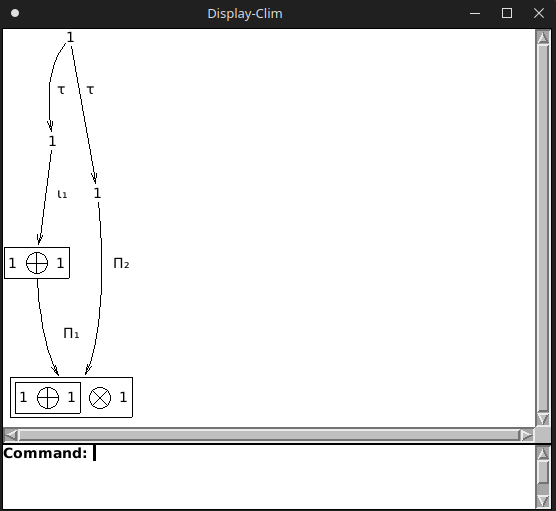
\includegraphics[scale=0.50]{images/SCRN.png}
\caption{Visualizer output for the compiled term \tcbox{pair (left so1 (unit))}}
\end{figure}

\end{document}
